    %% BioMed_Central_Tex_Template_v1.06
%%                                      %
%  bmc_article.tex            ver: 1.06 %
%                                       %

%%IMPORTANT: do not delete the first line of this template
%%It must be present to enable the BMC Submission system to
%%recognise this template!!

%%%%%%%%%%%%%%%%%%%%%%%%%%%%%%%%%%%%%%%%%
%%                                     %%
%%  LaTeX template for BioMed Central  %%
%%     journal article submissions     %%
%%                                     %%
%%          <8 June 2012>              %%
%%                                     %%
%%                                     %%
%%%%%%%%%%%%%%%%%%%%%%%%%%%%%%%%%%%%%%%%%


%%%%%%%%%%%%%%%%%%%%%%%%%%%%%%%%%%%%%%%%%%%%%%%%%%%%%%%%%%%%%%%%%%%%%
%%                                                                 %%
%% For instructions on how to fill out this Tex template           %%
%% document please refer to Readme.html and the instructions for   %%
%% authors page on the biomed central website                      %%
%% http://www.biomedcentral.com/info/authors/                      %%
%%                                                                 %%
%% Please do not use \input{...} to include other tex files.       %%
%% Submit your LaTeX manuscript as one .tex document.              %%
%%                                                                 %%
%% All additional figures and files should be attached             %%
%% separately and not embedded in the \TeX\ document itself.       %%
%%                                                                 %%
%% BioMed Central currently use the MikTex distribution of         %%
%% TeX for Windows) of TeX and LaTeX.  This is available from      %%
%% http://www.miktex.org                                           %%
%%                                                                 %%
%%%%%%%%%%%%%%%%%%%%%%%%%%%%%%%%%%%%%%%%%%%%%%%%%%%%%%%%%%%%%%%%%%%%%

%%% additional documentclass options:
%  [doublespacing]
%  [linenumbers]   - put the line numbers on margins

%%% loading packages, author definitions

%\documentclass[twocolumn]{bmcart}% uncomment this for twocolumn layout and comment line below
\documentclass{bmcart}

%%% Load packages
%\usepackage{amsthm,amsmath}
%\RequirePackage{natbib}
%\RequirePackage[authoryear]{natbib}% uncomment this for author-year bibliography
\RequirePackage{hyperref}
\usepackage[utf8]{inputenc} %unicode support
%\usepackage[applemac]{inputenc} %applemac support if unicode package fails
%\usepackage[latin1]{inputenc} %UNIX support if unicode package fails
\usepackage{graphicx}

\usepackage[noabbrev]{cleveref}
\usepackage{siunitx}
\DeclareSIUnit \basepair{bp}
\DeclareSIUnit \byte{B}
\DeclareSIPrefix\mebi{Mi}{10}
\DeclareSIPrefix\gibi{Gi}{10}

\usepackage{biocon}
\newplant{At}{genus=Arabidopsis,epithet=thaliana}

%%%%%%%%%%%%%%%%%%%%%%%%%%%%%%%%%%%%%%%%%%%%%%%%%
%%                                             %%
%%  If you wish to display your graphics for   %%
%%  your own use using includegraphic or       %%
%%  includegraphics, then comment out the      %%
%%  following two lines of code.               %%
%%  NB: These line *must* be included when     %%
%%  submitting to BMC.                         %%
%%  All figure files must be submitted as      %%
%%  separate graphics through the BMC          %%
%%  submission process, not included in the    %%
%%  submitted article.                         %%
%%                                             %%
%%%%%%%%%%%%%%%%%%%%%%%%%%%%%%%%%%%%%%%%%%%%%%%%%


%\def\includegraphic{}
%\def\includegraphics{}

\usepackage{todonotes}
\setlength{\marginparwidth}{3cm}

\newcounter{todocounter}
\newcommand{\ak}[1]
{\stepcounter{todocounter}
 \todo[color=green!40,author=Arthur]{\thetodocounter: #1}
 }


%%% Put your definitions there:
\startlocaldefs
\newcommand{\formatprogramnames}[1]{\texttt{#1}}
\newcommand{\ce}{\formatprogramnames{chloroExtractor}}
\newcommand{\oa}{\formatprogramnames{ORG.Asm}}
\newcommand{\fp}{\formatprogramnames{Fast-Plast}}
\newcommand{\ioga}{\formatprogramnames{IOGA}}
\newcommand{\np}{\formatprogramnames{NOVOPlasty}}
\newcommand{\go}{\formatprogramnames{GetOrganelle}}
\newcommand{\cassp}{\formatprogramnames{Chloroplast assembly protocol}}

\newcommand{\zenododataset}{\cite{zenododataset}}
\newcommand{\zenodorepo}{\cite{zenodorepo}}

% Niklas table
%\newcommand{\ok}{\textcolor[rgb]{0.7,0.7,0}{\textsc{\bfseries{}OKAY}}}
%\newcommand{\bad}{\textcolor{red}{\textsc{\bfseries{}BAD}}}
%\newcommand{\good}{\textcolor[rgb]{0,0.6,0}{\textsc{\bfseries{}GOOD}}}
\newcommand{\ok}{\textsc{Okay}}
\newcommand{\bad}{\textsc{Bad}}
\newcommand{\good}{\textsc{Good}}


% List of docker images
\newcommand{\docker}[2]{\href{https://cloud.docker.com/u/chloroextractorteam/repository/docker/chloroextractorteam/#1}{chloroextracteam/#1:#2}}
\newcommand{\dockerce}{\docker{benchmark\_chloroextractor}{v2.0.0}}
\newcommand{\dockercesha}{\texttt{8f49e03424b37e699c5fea9391f79dbb9f2d0dc550ce86c4c700f39deec2dacd}}
\newcommand{\dockeroa}{\docker{benchmark\_org-asm}{v2.0.0}}
\newcommand{\dockeroasha}{\texttt{ff83677c97b7c4e346191b9e04a5162eeea2a8dfd9e60ff84067d33747868f60}}
\newcommand{\dockerfp}{\docker{benchmark\_fastplast}{v2.0.0}}
\newcommand{\dockerfpsha}{\texttt{a3d06a610f8340ba49c3ff3b27342534e2a5348b17caa4fd3c3f3d327243a272}}
\newcommand{\dockerioga}{\docker{benchmark\_ioga}{v2.0.0}}
\newcommand{\dockeriogasha}{\texttt{4698a21c343c60290bbf16811165a654ff01e8fddeb41cd75d0771b7f45968c0}}
\newcommand{\dockernp}{\docker{benchmark\_novoplasty}{v2.0.0}}
\newcommand{\dockernpsha}{\texttt{106387bad4e8e5c53fb9d4c3bdd60cdddf05a47b52a38697369eeabb947c547c}}
\newcommand{\dockergo}{\docker{benchmark\_getorganelle}{v2.0.0}}
\newcommand{\dockergosha}{\texttt{2ed3a464a82025a196ea56c649d0b0a3472cef76994bb065d56054d93298d956}}
\newcommand{\dockercassp}{\docker{benchmark\_chloroplast\_assembly\_protocol}{v2.0.0}}
\newcommand{\dockercasspsha}{\texttt{d10d2317103d91fadec4cb1d5466ac109f23176ad74b6f44f0179175f050155d}}
\endlocaldefs


%%% Begin ...
\begin{document}

%%% Start of article front matter
\begin{frontmatter}

\begin{fmbox}
\dochead{Research}

%%%%%%%%%%%%%%%%%%%%%%%%%%%%%%%%%%%%%%%%%%%%%%
%%                                          %%
%% Enter the title of your article here     %%
%%                                          %%
%%%%%%%%%%%%%%%%%%%%%%%%%%%%%%%%%%%%%%%%%%%%%%

\title{The landscape of chloroplast genome assembly tools}

%%%%%%%%%%%%%%%%%%%%%%%%%%%%%%%%%%%%%%%%%%%%%%
%%                                          %%
%% Enter the authors here                   %%
%%                                          %%
%% Specify information, if available,       %%
%% in the form:                             %%
%%   <key>={<id1>,<id2>}                    %%
%%   <key>=                                 %%
%% Comment or delete the keys which are     %%
%% not used. Repeat \author command as much %%
%% as required.                             %%
%%                                          %%
%%%%%%%%%%%%%%%%%%%%%%%%%%%%%%%%%%%%%%%%%%%%%%

\author[
    addressref={aff2,aff3},
    noteref={n1},
    email={jan.freudenthal@uni-wuerzburg.de}
    ]{\inits{JAF}\fnm{Jan A} \snm{Freudenthal}}
\author[
    addressref={aff2},
    noteref={n1},
    email={simon-pfaff@gmx.de}
    ]{\inits{SP}\fnm{Simon} \snm{Pfaff}}
\author[
   addressref={aff1,aff3},
   email={niklas.terhoeven@uni-wuerzubrg.de}
]{\inits{NT}\fnm{Niklas} \snm{Terhoeven}}
\author[
   addressref={aff1,aff2,aff3 },
   noteref={n2},
   email={markus.ankenbrand@uni-wuerzubrg.de}
]{\inits{MJA}\fnm{Markus J} \snm{Ankenbrand}}
\author[
   addressref={aff1,aff4},                   % id's of addresses, e.g. {aff1,aff2}
   corref={aff1},                       % id of corresponding address, if any
   noteref={n2},                        % id's of article notes, if any
   email={frank.foerster@uni-wuerzburg.de}   % email address
]{\inits{FF}\fnm{Frank} \snm{Förster}}


%%%%%%%%%%%%%%%%%%%%%%%%%%%%%%%%%%%%%%%%%%%%%%
%%                                          %%
%% Enter the authors' addresses here        %%
%%                                          %%
%% Repeat \address commands as much as      %%
%% required.                                %%
%%                                          %%
%%%%%%%%%%%%%%%%%%%%%%%%%%%%%%%%%%%%%%%%%%%%%%

\address[id=aff2]{%                           % unique id
  \orgname{Department of Bioinformatics, University of W\"{u}rzburg}, % university, etc
  \street{Biozentrum, Am Hubland},                     %
  \postcode{97074},                                % post or zip code
  \city{W\"{u}rzburg},                              % city
  \cny{Germany}                                    % country
}
\address[id=aff1]{%
  \orgname{Center for Computational and Theoretical Biology, University of W\"{u}rzburg},
  \street{Campus Hubland Nord},
  \postcode{97074}
  \city{W\"{u}rzburg},
  \cny{Germany}
}
\address[id=aff3]{%
  \orgname{AnaLife Data Science},
  \street{Friedrich-Bergius-Ring 15},
  \postcode{97076}
  \city{W\"{u}rzburg},
  \cny{Germany}
}
\address[id=aff4]{%
  \orgname{Fraunhofer IME-BR},
  \street{Winchester Str.\ 2},
  \postcode{97076}
  \city{Gie\ss{}en},
  \cny{Germany}
}

%%%%%%%%%%%%%%%%%%%%%%%%%%%%%%%%%%%%%%%%%%%%%%
%%                                          %%
%% Enter short notes here                   %%
%%                                          %%
%% Short notes will be after addresses      %%
%% on first page.                           %%
%%                                          %%
%%%%%%%%%%%%%%%%%%%%%%%%%%%%%%%%%%%%%%%%%%%%%%

\begin{artnotes}
%\note{Sample of title note}     % note to the article
\note[id=n1]{Equal contributor} % note, connected to author
\note[id=n2]{Corresponding author} % note, connected to author
\end{artnotes}

\end{fmbox}% comment this for two column layout

%%%%%%%%%%%%%%%%%%%%%%%%%%%%%%%%%%%%%%%%%%%%%%
%%                                          %%
%% The Abstract begins here                 %%
%%                                          %%
%% Please refer to the Instructions for     %%
%% authors on http://www.biomedcentral.com  %%
%% and include the section headings         %%
%% accordingly for your article type.       %%
%%                                          %%
%%%%%%%%%%%%%%%%%%%%%%%%%%%%%%%%%%%%%%%%%%%%%%

\begin{abstractbox}

\begin{abstract} % abstract
The special issue will accept manuscripts presenting:

- in-depth analyses of advantages

-limitations of state-of-the-art methods

-demonstration on a variety of representative datasets and simulations

-clear guidelines/recommendations for the end-user

-insight into future directions for methods
\parttitle{First part title} %if any
Text for this section.

\parttitle{Second part title} %if any
Text for this section.
\end{abstract}

%%%%%%%%%%%%%%%%%%%%%%%%%%%%%%%%%%%%%%%%%%%%%%
%%                                          %%
%% The keywords begin here                  %%
%%                                          %%
%% Put each keyword in separate \kwd{}.     %%
%%                                          %%
%%%%%%%%%%%%%%%%%%%%%%%%%%%%%%%%%%%%%%%%%%%%%%

\begin{keyword}
\kwd{Chloroplast}
\kwd{Genome assembly}
\kwd{author}
\end{keyword}

% MSC classifications codes, if any
%\begin{keyword}[class=AMS]
%\kwd[Primary ]{}
%\kwd{}
%\kwd[; secondary ]{}
%\end{keyword}

\end{abstractbox}
%
%\end{fmbox}% uncomment this for twcolumn layout

\end{frontmatter}

%%%%%%%%%%%%%%%%%%%%%%%%%%%%%%%%%%%%%%%%%%%%%%
%%                                          %%
%% The Main Body begins here                %%
%%                                          %%
%% Please refer to the instructions for     %%
%% authors on:                              %%
%% http://www.biomedcentral.com/info/authors%%
%% and include the section headings         %%
%% accordingly for your article type.       %%
%%                                          %%
%% See the Results and Discussion section   %%
%% for details on how to create sub-sections%%
%%                                          %%
%% use \cite{...} to cite references        %%
%%  \cite{koon} and                         %%
%%  \cite{oreg,khar,zvai,xjon,schn,pond}    %%
%%  \nocite{smith,marg,hunn,advi,koha,mouse}%%
%%                                          %%
%%%%%%%%%%%%%%%%%%%%%%%%%%%%%%%%%%%%%%%%%%%%%%

%%%%%%%%%%%%%%%%%%%%%%%%% start of article main body
% <put your article body there>

%%%%%%%%%%%%%%%%
%% Background %%
%%
\newpage
\section*{Introduction}
\subsection*{General introduction and motivation}
The chloroplast as the photosynthetic organelle harboring its own genome has been an early target for sequencing.\ak{maybe even 1-2 sentences about general chloroplast importance}
The first chloroplast genome sequences were obtained as early as 1986 \cite{ohyama_chloroplast_1986,shinozaki_complete_1986}.
These efforts elucidated the general genome organization and structure of chloroplasts, expanded by many more studies over the years.
Chloroplast genome content and structure \textcolor{red} {are}  reviewed elsewhere \cite{wicke_evolution_2011,green_chloroplast_2011}.
Chloroplast genomes are widely used for evolutionary analyses \cite{martin_plastid_2010,xiao-ming_inferring_2017}, barcoding \cite{kress_use_2005,hollingsworth_dna_2009,de_vere_dna_2015}, and meta-barcoding \cite{bell_review_2016,deiner_environmental_2017}.
Interesting aspect of chloroplast genomes are their reduced size through endosymbiotic gene transfer \cite{martin_evolutionary_2002,timmis_endosymbiotic_2004} and the strong conservation of the remaining genes (cite).
Despite the overall high conservation there are striking differences between groups (e.g. loss of whole gene families like ndh genes in \textit{Droseraceae} \cite{nevill_plastome-wide_2019} and extreme evolutionary cases with very low GC content and a modified genetic code \cite{su_novel_2019}).
These differences call for comparative genomic approaches.

It is much easier to decipher the complete chloroplast genome than the complete core genome, due its comparably smaller size. For example \textit{Arabidopsis thaliana} core genome is approximately \SI{125}{\mega\basepair} in length \cite{schmuths2004,cao2011} while the size of the chloroplast genome with \SI{154}{\kilo\basepair} is more than \SI{800}{\times} smaller than the core genome \cite{sato1999}.    
However, the specific genome structure (esp. the large inverted repeat) complicates automated resolution with short read technologies (cite?).
Many genome sequencing projects contain chloroplast reads as by-product.
In some cases the chloroplast data is even considered contamination so experimental protocols for reducing their content have been developed \cite{lutz_isolation_2011}.
The resolved chloroplast genome helps to remove these reads, which can improve assembly of the core genome.
Databases exist, containing short read data for species where no reference chloroplast is publicly available.
There is a lot of potential use cases for chloroplast genomes \cite{tonti-filippini_what_2017}
Resolving these (hidden treasures) would allow for more and larger scale comparative studies on whole chloroplasts.
In a different application researchers use shallow genome sequencing to reconstruct full chloroplast genomes for use as super-barcodes \cite{coissac_barcodes_2016}.
There are also applications in biotechnology and genetic engineering \cite{daniell_chloroplast_2016}.

\subsection*{Chloroplast genome architecture}
Maybe separate section describing a prototypical chloroplast: LSC, IRa, SSC, IRb. Gene number and content. Size ranges. Evolutionary history incl. endosymbiontic gene transfer. Reduced genomes in parasitic plants. Loss of ndh gene family (maybe too specific). Preliminary SNP analysis in \plant{At} to estimate intraspecific variability? Is there anything known about intra-organismic variability (do some plants have multiple populations of chloroplasts? \ak{Yes, they do , Heteroplasmy} probably off topic).\ak{nope, I think this is important}

\subsection*{Approaches to extracting chloroplasts from whole genome data}
\todo{ausbauen}
1. Getting chloroplast reads out of mixed files
Mapping (potentially iterative), k-mer coverage analysis, seeded assembly
2. Assembly of chloroplast (incl special structure with IRs)
normal assembly - then blast, assembly then graph resolution, might be combined with step 1.
\cite{twyford_strategies_2017}

\subsection*{Purpose and scope of this study}
The goal of this study is to compare the effectiveness and efficiency of existing open source command-line tools to de-novo assemble whole chloroplast genomes from raw mixed genomic data sets with minimal configuration.
This means: no data preparation, no specific reference (but \plant{At} if required), default parameters, no manual finishing.
We further restricted our benchmark to paired Illumina data sets as these are the most common \todo{cite?} and the %\todo{(all?) - habs gecheckt}
tools in this study can not handle any other types.

In our opinion this reflects the most common use cases: (1) a user trying a tool quickly without digging into options for fine tuning and (2) large scale automatic applications.
Still, we acknowledge that the performance of the tools might be significantly improved by optimizing parameters (and references if applicable) for each data set specifically.
(However, this was outside the scope of this study.)

%Clearly state criteria. Work with mixed data. Full automation. De novo - no manual selection of appropriate reference. No manual finishing. The step we are interested in is: from raw paired Illumina (!) reads to a fasta file containing the assembly (optimally full, circularized and on one contig). We are not interested in annotation or any additional contigs (genomic, mitochondrion, rRNA, etc.).
%\cite{koon,oreg,khar,zvai,xjon,schn,pond,smith,marg,hunn,advi,koha,mouse}

\section*{Methods}
Source code for all methods is available at \url{https://github.com/chloroExtractorTeam/benchmark} and archived under \zenodorepo{}.
All docker images are published on \url{https://cloud.docker.com/u/chloroextractorteam/} and are named with a leading \texttt{benchmark\_} (\cref{tab:dockerimages}).
Our simulated data sets are stored at \zenododataset{}.
This study adheres to the guidelines for computational method benchmarking \cite{weber_essential_2018}.

\subsection*{Tool Selection}

We included tools designed for assembling chloroplasts from whole genome paired end Illumina sequencing data. The tools must be available as open source software and allow execution via a command line interface. A graphical user interface is not suitable for
running automated comparisons. The following tools were determined to be within the scope of this study:

\oa{} \cite{coissac_barcodes_2016}, 
\ce{} \cite{j_ankenbrand_chloroextractor:_2018}, 
\fp{} \cite{mckain__fast-plast_2017}, 
\ioga{} \cite{bakker_herbarium_2016}, 
\np{} \cite{dierckxsens_novoplasty:_2017}, 
\go{} \cite{jin_getorganelle:_2018}, 
\cassp{} \cite{sancho_comparative_2018}.

Other related tools for assembling chloroplasts but outside the scope of this study are \texttt{Organelle PBA} \cite{Soorni2017}, \texttt{sestaton/Chloro} \cite{sestaton}, \texttt{Norgal}  \cite{Al-Nakeeb2017} and \texttt{MitoBim} \cite{mitobim2013}.

\texttt{Organelle PBA} is designed for PacBio data and does not work with paired Illumina data only.
\texttt{sestaton/Chloro} fits all criteria but is flagged as a work in progress and development seems to have ended two years ago.
\texttt{Norgal} is a tool to extract organellar DNA from whole genome data based on a k-mer frequency approach. However the final output is a set of contigs of mixed mitochondrial and plastid origin. The suggested approach to get a finished chloroplast genome is to run \np{} on the ten longest contigs.
\texttt{MitoBim} is specifically designed for mitochondrial genomes. Even though there is a claim by the author that it can be used for chloroplasts as well (\url{https://github.com/chrishah/MITObim/issues/16}, accessed: 2019-05-27), there is no further description on how to do that. \todo{haben wir es versucht? - nein}
Additionally, there is a protocol for the \texttt{Geneious} \cite{geneious} software available \cite{geneious-protocol}.
However, \texttt{Geneious} is closed source and GUI based, which is not in the scope of this study.
There is also another publication describing a method for assembling chloroplasts \cite{method-description-paper}. However, the link to the software is not active anymore.


\subsection*{Our Setup}
\todo{ausformulieren}
Defined interface, forward.fq and reverse.fq as only input. output.fa as only relevant output.
Docker container, all derived from main container, wrapper script makes all tools work conforming to the defined interface. Run docker containers for performance measurement and singularity containers on real datasets.
Singularity container were built from docker containers for usage on Julia-HPC of JMU using Singularity v.2.5.2 \cite{kurtzer2017singularity}
All singularity containers were run on the Julia-HPC on Intel® Xeon® Gold \num{6140} Processors using slurm workload manager version 17.11.8 \cite{Jette02slurm}. Assemblies run on \num{4} threads using \SI{10}{\gibi\byte} RAM with a timelimit of \SI{48}{\hour}. 
\subsection*{Data}
\subsubsection*{Simulated}
To avoid suffering from sequencing errors and biological variances, we simulated perfect reads based on the \plant{At} (TAIR10) chloroplast assembly \cite{tair10}.
Therefore we used a sliding window approach with seqkit \cite{seqkit}. The exact commands can be found inside \href{https://github.com/chloroExtractorTeam/benchmark/blob/master/03_representative_datasets.md}{\texttt{03\_representative\_datasets.md}} in \zenododataset{}.
For the final simulated data sets reads based on pseudo mixtures of TAIR10's core and chloroplast genome:  \num{0}:\num{1}, \num{1}:\num{10}, \num{1}:\num{100}, and \num{1}:\num{1000}.
Additionally, we generated different read lengths (\SIlist{150;250}{\basepair}).

%(circular for chloro and mito). No errors, no insert size variation, perfect quality, equal coverage.

\subsubsection*{Real}
We downloaded sequencing data from SRA \cite{sra2010} of all organisms with a reference
chloroplast in CpBase \cite{cpbase}. In total, this accumulated to \num{380} datasets, including \num{6} without data and \num{5} with malformatted data. This leads to a total set of \num{369} datasets \todo{see supplementary table?}.

\subsection*{Evaluation Criteria}
\subsubsection*{Computational Resources}
Due to computational resources are limited, we evaluated the effect of different input parameters.
To monitor the influence, we recorded the mean and the peak CPU usage, the peak memory consumption, and the size of the assembly folder. 
As input data, we used different data sets comprising \numlist{25000;250000;2500000} read pairs based on our simulated perfect reads.
Therefore, the simulated perfect read files have been read repeatedly to achieve the required number of read pairs.
We used our docker image setup (\cref{tab:dockerimages}) to run all assembly programs three times on a given parameter setting.
The setting combined the different input data and different number of threads to use (\numlist{1;2;4;8}).
Some programs used more CPU threads than specified, therefore, the number of CPUs available have been fixed using the CPUs option while running the docker run command.
For each assembly setting, we recorded the peak memory consumption, the CPU usage for calculation of mean and peak CPU usage, and the size of the folder where the assembly was calculated.
The values of CPU and memory usage have been obtained by docker.
The disk usage was estimated using the GNU tool \texttt{du}.
We used \texttt{GNU parallel} for queuing of the different settings \cite{Tange2011a}.

\subsubsection*{Qualitative}

The qualitative evaluation is mainly based on the reviewer guidelines for the Journal of Open Source Software (JOSS) \cite{joss}.
To create a standard environment, all tools were tested in a fresh default installation of Ubuntu 18.04.2 running in a virtual machine (VirtualBox Version 5.2.18\_Ubuntu r123745). We chose this setup instead of the docker container, because it resembles a typical user environment better than the minimal docker installation. The tools were installed according to their installation instructions and
the provided tutorial or example usage was executed. During the evaluation, the following
questions were asked:

\begin{itemize}
    \item Is the tool easy to install? 
    \item Is there a way to test the installation or a tutorial on how to use the tool? 
    \item Is there a good documentation on the parameter settings? 
    \item Is the tool maintained (issues answered, implementation of new features)? 
    \item Is the tool Open Source?
\end{itemize}

These questions were answered with \good{}, \ok{} or \bad{}, depending on the quality of the result. 
For example, a \good{} installation utilizes a automated package or dependency management like apt,
CRAN, docker, etc. An \ok{} installation procedure provides a custom script to install everything
or at least lists all dependencies. A \bad{} installation procedure fails to list important dependencies
or produces errors, that prevent a successful installation. 

After an initial evaluation, we contacted all authors via their GitHub or GitLab issue tracking to
report any flaws we found.

\subsubsection*{Quantitative}

%We use continuity: number of contigs.
%Completeness: Number of covered bases on reference (when aligning assembly).
%Correctness: Number of covered bases in assembly (when aligning reference).
%Repeat resolution: Difference between above two measures (indicates collapsed or expanded repeats)
%
%\nocite{oreg,schn,pond,smith,marg,hunn,advi,koha,mouse}


%We want to quantify continuity, completeness, correctness and repeat resolution.

Foreach dataset and assembler the proposed chloroplast was compared to the respective reference chloroplast using a pairwise alignment obtained with \texttt{minimap2} v2.16 \cite{li2018minimap2}. Based on theses alignments the score is calculated as shown in \cref{eq:quantitative}
The assemblies were scored on a scale from 0 to 100, with 100 being the best and 0 the worst possible score. Four different metrics were Incorporated, each contributing  $\frac{1}{4}$ to the total score: Completeness, correctness, repeat resolution and continuity.

The completeness is estimated as the coverage of the assembled chloroplast genome versus the reference genome ($cov_{ref}$). It resembles how many bases of the query genome can be mapped to its respective reference genome. Secondly, we mapped the reference genome against the query. The coverage of the reference genome ($cov_{qry}$) is used as measurment for the correctness of the assembly. The repeat resolution is estimated from the size difference of the assembly and the reference genome ($min\left\{ \frac{cov_{qry}}{cov_{ref}}, \frac{cov_{ref}}{cov_{qry}}\right\}$).The $min$ was applied to ensure, that only values between 0 and 1 were obtained. The fourth metric used is the continuity, represented by the number of contigs. A perfect score is achieved if one circular chromosome was assembled.



\begin{equation}
   score = \frac{1}{4} \cdot \left( cov_{ref} +  cov_{qry} + min\left\{ \frac{cov_{qry}}{cov_{ref}}, \frac{cov_{ref}}{cov_{qry}}\right\} + \frac{1}{n_{contigs} }\right) \cdot 100 
   \label{eq:quantitative}
\end{equation}



\subsubsection*{Reproducibility}
For reproducibility  testing we randomly choose  \num{100} data sets, that in the previous runs resulted in outputs for most of the assemblers and run them again with the same parameters as before. The resulting assemblies were scored again as described above and the scores of the 1. and the 2. run were compared to each other. 

\section*{Results}
\subsection*{Performance metrics}
%\subsection*{Computational Resources}
%Table and figure of performance evaluation. Including RAM, I/O, runtime, parallelization ability, CPU usage. Free text description of results, range, mean/median, effect of input size, threads parameter, ...

\subsubsection*{Time requirements}
In terms of time efficiency there was a great difference between input datasets, number of threads and the tool in use ranging from a few minutes to several hours (\cref{fig:performance_runtime}).
Some assemblies failed to finish within the time-limit we set at \SI{48}{\hour}. 
On average the longest time to complete assemblies was taken by \ioga{} and \fp{} followed by \oa{} and \go{} the most time efficient overall was \ce{} with on average is a little faster than \np{} and \cassp{}.
%% multithreading
Not all the tools were able to benefit from having access to multiple threads. Both \np{} and \oa{} take about the same time independent of being able to utilize \numlist[list-final-separator={, or }]{1;2;4;8} threads. \cassp{}, \ce{} , \go and \fp{} all profit from multi-threading (\cref{fig:performance_runtime}, \cref{fig:performance_memory_cpu}).

\subsubsection*{Memory and CPU Usage }
The peak and mean CPU usage, as well as peak memory and disk usage have been recorded for all assemblers based on a input data set size and a number of threads to use (\cref{fig:performance_memory_cpu}).
Mainly, the size of the input set influenced the peak memory usage with an exception for \ce{} and \ioga{}.
Those two assemblers seems to have a memory usage pattern, which is less influenced by data set size.
The number of allowed threads have only no or a limited impact on the peak memory usage.
Nevertheless, all programs profit by a higher number of threads, even more if the input size increases.
In contrast, the disk usage is independent from input size and number of threads for all assemblers, but the factor between the programs exceeds a factor of \num{100}.

\subsection*{Qualitative}
Most of the tools were evaluated as mainly \good{} (see table \ref{tab:resultsQual}). However, a few critique points remained.
Two minor dependencies were missing in the \go{} installation instructions. There was also no test data available and an issue occurred when running it on a \plant{At} data set. We are currently in the process of resolving this with the authors.

The \fp{} installation instructions were missing some dependencies. Like \go{}, \fp{} does not offer a test data set or a tutorial, except from some example commands. 

The \oa{} installation instructions did not work. We found some issues, which are probably related to the requirement of \texttt{Python~3.7}. There is a tutorial with sample data available. However following the instructions resulted in a segmentation fault. We found a workaround for this bug and contacted the authors.

The main critique point of \np{} was the lack of a test data set with instructions. This was fixed by the authors after we contacted them. \np{} uses a custom license. An OSI approved license would be preferred here.

The \ce{} does come with a test data set and a short tutorial. However, a way to evaluate the results of the test run would be nice.

The \ioga{} installation instructions were missing many dependencies. Also, there was no test data or tutorial available and there is no license assigned to it. Since there was no update to the GitHub repository for the last three years, the project can be seen as inactive. After contact, the authors promised to resolve the mentioned issues.

As many of the other tools, the installation instructions for the \cassp{} were missing some dependencies. The list was updated after we contacted the authors. This tool does come with a test data set, however a note about the expected outcome would be nice. A more extensive tutorial is provided. The description about the parameter is short, but seems to be sufficient.

\subsection*{Quantitative}
\subsubsection*{Simulated data}
The only assembler obtaining perfect results according to our score for the simulated data sets is \go{} (\cref{fig:simulated}).
\ioga{} and \cassp{} showed the worst performance being unable to fully assemble a single chloroplast out of \num{14}.
\np{} performed second best with scores above \num{80} for all data sets, only failing to resolve the chloroplast contig into one single circular assembly.
(As could have been expected -> discussion) the overall performance is best, when the input data consists purely of chloroplast reads.
Only \ioga{} and \cassp{} failed to deliver any results once each.
Besides that no clear causality between length of the input reads, ratio of core vs chloroplast reads and the performance can be clearly observed. 

\subsubsection*{real data sets}
Concerning the performance of the assemblers on evaluated on the real data sets from SRA database we were able to observe considerable differences in the median score (\cref{fig:swarmplot}).
The highest scores were achieved by \go{} with a median of 99.7 and 199 circular assemblies out of a total of 356 assemblies that resulted in an output  \cref{tab:scores}.
The performance of \go{} is seconded by \fb{} \np{} \oa{}, with \fb{} outperforming the latter two slightly in terms of score, however \fb{} as almost or more than twice as much \num{114} perfectly assembled chloroplast genomes as \np{} with \num{66} or \num{55} circular genomes for \oa{}.
\ioga{} and \cassp{} were both not able to assemble a single circular, single-contig genome \cref{tab:scores}, consequently resulting in the lowest mean and median scores.  



%% Ich werde die Namen in der Tabelle anpassen, sobald ich die finale Version habe 

\cref{fig:upset}

\textit{swarm plot goes here}
%% Den upset plot eventuell erst in die Discussion reinbringen ? Da wir davon ableiten welche tools wir empfehlen?


\subsubsection*{Reproducibility}
Reproducibility was tested as described above, by re-running assemblies and comparison of the scores of the two assemblies (\cref{fig:reproducibility}).
Replicates that did not produce an output were manually scored with \num{0}. 
\go{} was the only tool that succeeded in obtaining similar scores for all the assemblies, without having and completely unsuccessful assemblies for this subset of data. Except for \fp{} all the other tools had at least one assembly that was unsuccessful in either runs, but produced an output in the other.  Notably \ioga{} appears to have a tendency of being able to perform differently in independent runs. More that \SI{10}{\percent} of the assemblies failed once, but were successful in the other run.

Both \fp{} and \np{} tend to have minor changes in the assembly when the overall performance is comparably well, leading to the arrow-shaped scatter plots. \ce{} and \cassp{} only have few deviations between the two runs, besides a few one-time non-performing data sets, the other all scored the same.

\section*{Discussion}
Discuss Computational Resources. Implications of very long running. Also state minimum requirements on the hardware (RAM, CPUs, storage). Importance of this depends on use case (if goal is one single chloroplast 

We evaluated all tools under the assumption that they are used in the most basic form (default parameters, no hand selected reference, no pre-processing of the data or post-processing of the result, restricted runtime). It is important to note that any tool might perform significantly different if parameters and references are fine-tuned for each data set.

\subsection*{Clear guidelines for the end-user}
Which program (or combination of programs) to use? Does the decision depend on some parameter of the data (read length, amount, taxonomic group, ...)?

\subsection*{Ideas for future development}
Combining components from different tools might be a promising approach. E.g. read scaling from \ce{}, assembly from \go{} and structural resolution with \fp{}.
Mitigate installation issues e.g. by containerization.
Improve documentation and usability.
Maybe better integrated guessing of parameters (?) at least for automatization (but also because users tend to run a tool with default settings and look on what they get, only powerusers tweak parameters - and if it is possible to get a full chloroplast by guessing the best parameters there is no need for specific knowledge of parameters and their effects by the end user).
Other (more) data types, PacBio, nanopore.

\section*{Conclusion}
%Short summary of clear guidelines and future development (might not be necessary as these are the last two sections of the Discussion anyway, so we might elect to skip this).
\todo{sollten wir lobend erwähnen, dass alle auf github/gitlab sind?}

Put results back in context: the multitude of available tools shows importance to solve the challenge of chloro extraction. Presented benchmarking shows that all tools sometimes struggle even with ``perfect'' data. Although no program works everytime, most chloroplasts are resolved by at least one tool (is that so?). So programs are complementary, more effort to combine strengths of different methods (or automatic parameter selection - if failure is due to suboptimal parameters for the specific data set).

Outlook: next step in the pipeline is annotation. There is a similar problem: many tools, which one to use? 
A large scale study reconstructing chloroplasts throughout SRA (or \num{1001} genome project) is feasible and promising using the existing tools (estimated runtime, number of novel chloroplasts).
A meta-tool that automatically combines the different programs could be developed.
The benchmarking study could be augmented to automatically select the closest reference from the database and provide that to any tool that can take advantage of references.

%%%%%%%%%%%%%%%%%%%%%%%%%%%%%%%%%%%%%%%%%%%%%%
%%                                          %%
%% Backmatter begins here                   %%
%%                                          %%
%%%%%%%%%%%%%%%%%%%%%%%%%%%%%%%%%%%%%%%%%%%%%%

\begin{backmatter}

\section*{Competing interests}
  The authors disclose that SP, NT, FF, and MJA are developers of \ce{}, one of the tools benchmarked in this article. The authors exercised caution not to let this fact unfairly influence their judgment.

\section*{Author's contributions}
MJA and FF conceived of the presented idea and supervised the findings of this manuscript.
SP and FF created the docker images.
NT performed the qualitative analysis for all assemblers.
MJA prepared the simulated and real data sets.
JAF assembled the real data sets.
FF ran the performance assemblies on the simulated data sets.
All authors developed the score model.
JAF and MJA implemented the score model and prepared the figures.
All authors discussed the results and contributed to the final manuscript.

\section*{Acknowledgements}
  Text for this section \ldots
%%%%%%%%%%%%%%%%%%%%%%%%%%%%%%%%%%%%%%%%%%%%%%%%%%%%%%%%%%%%%
%%                  The Bibliography                       %%
%%                                                         %%
%%  Bmc_mathpys.bst  will be used to                       %%
%%  create a .BBL file for submission.                     %%
%%  After submission of the .TEX file,                     %%
%%  you will be prompted to submit your .BBL file.         %%
%%                                                         %%
%%                                                         %%
%%  Note that the displayed Bibliography will not          %%
%%  necessarily be rendered by Latex exactly as specified  %%
%%  in the online Instructions for Authors.                %%
%%                                                         %%
%%%%%%%%%%%%%%%%%%%%%%%%%%%%%%%%%%%%%%%%%%%%%%%%%%%%%%%%%%%%%

% if your bibliography is in bibtex format, use those commands:
\bibliographystyle{bmc-mathphys} % Style BST file (bmc-mathphys, vancouver, spbasic).
\bibliography{bmc_article}      % Bibliography file (usually '*.bib' )
% for author-year bibliography (bmc-mathphys or spbasic)
% a) write to bib file (bmc-mathphys only)
% @settings{label, options="nameyear"}
% b) uncomment next line
%\nocite{label}

% or include bibliography directly:
% \begin{thebibliography}
% \bibitem{b1}
% \end{thebibliography}

%%%%%%%%%%%%%%%%%%%%%%%%%%%%%%%%%%%
%%                               %%
%% Figures                       %%
%%                               %%
%% NB: this is for captions and  %%
%% Titles. All graphics must be  %%
%% submitted separately and NOT  %%
%% included in the Tex document  %%
%%                               %%
%%%%%%%%%%%%%%%%%%%%%%%%%%%%%%%%%%%

%%
%% Do not use \listoffigures as most will included as separate files

\section*{Figures}
  \begin{figure}[h!]
  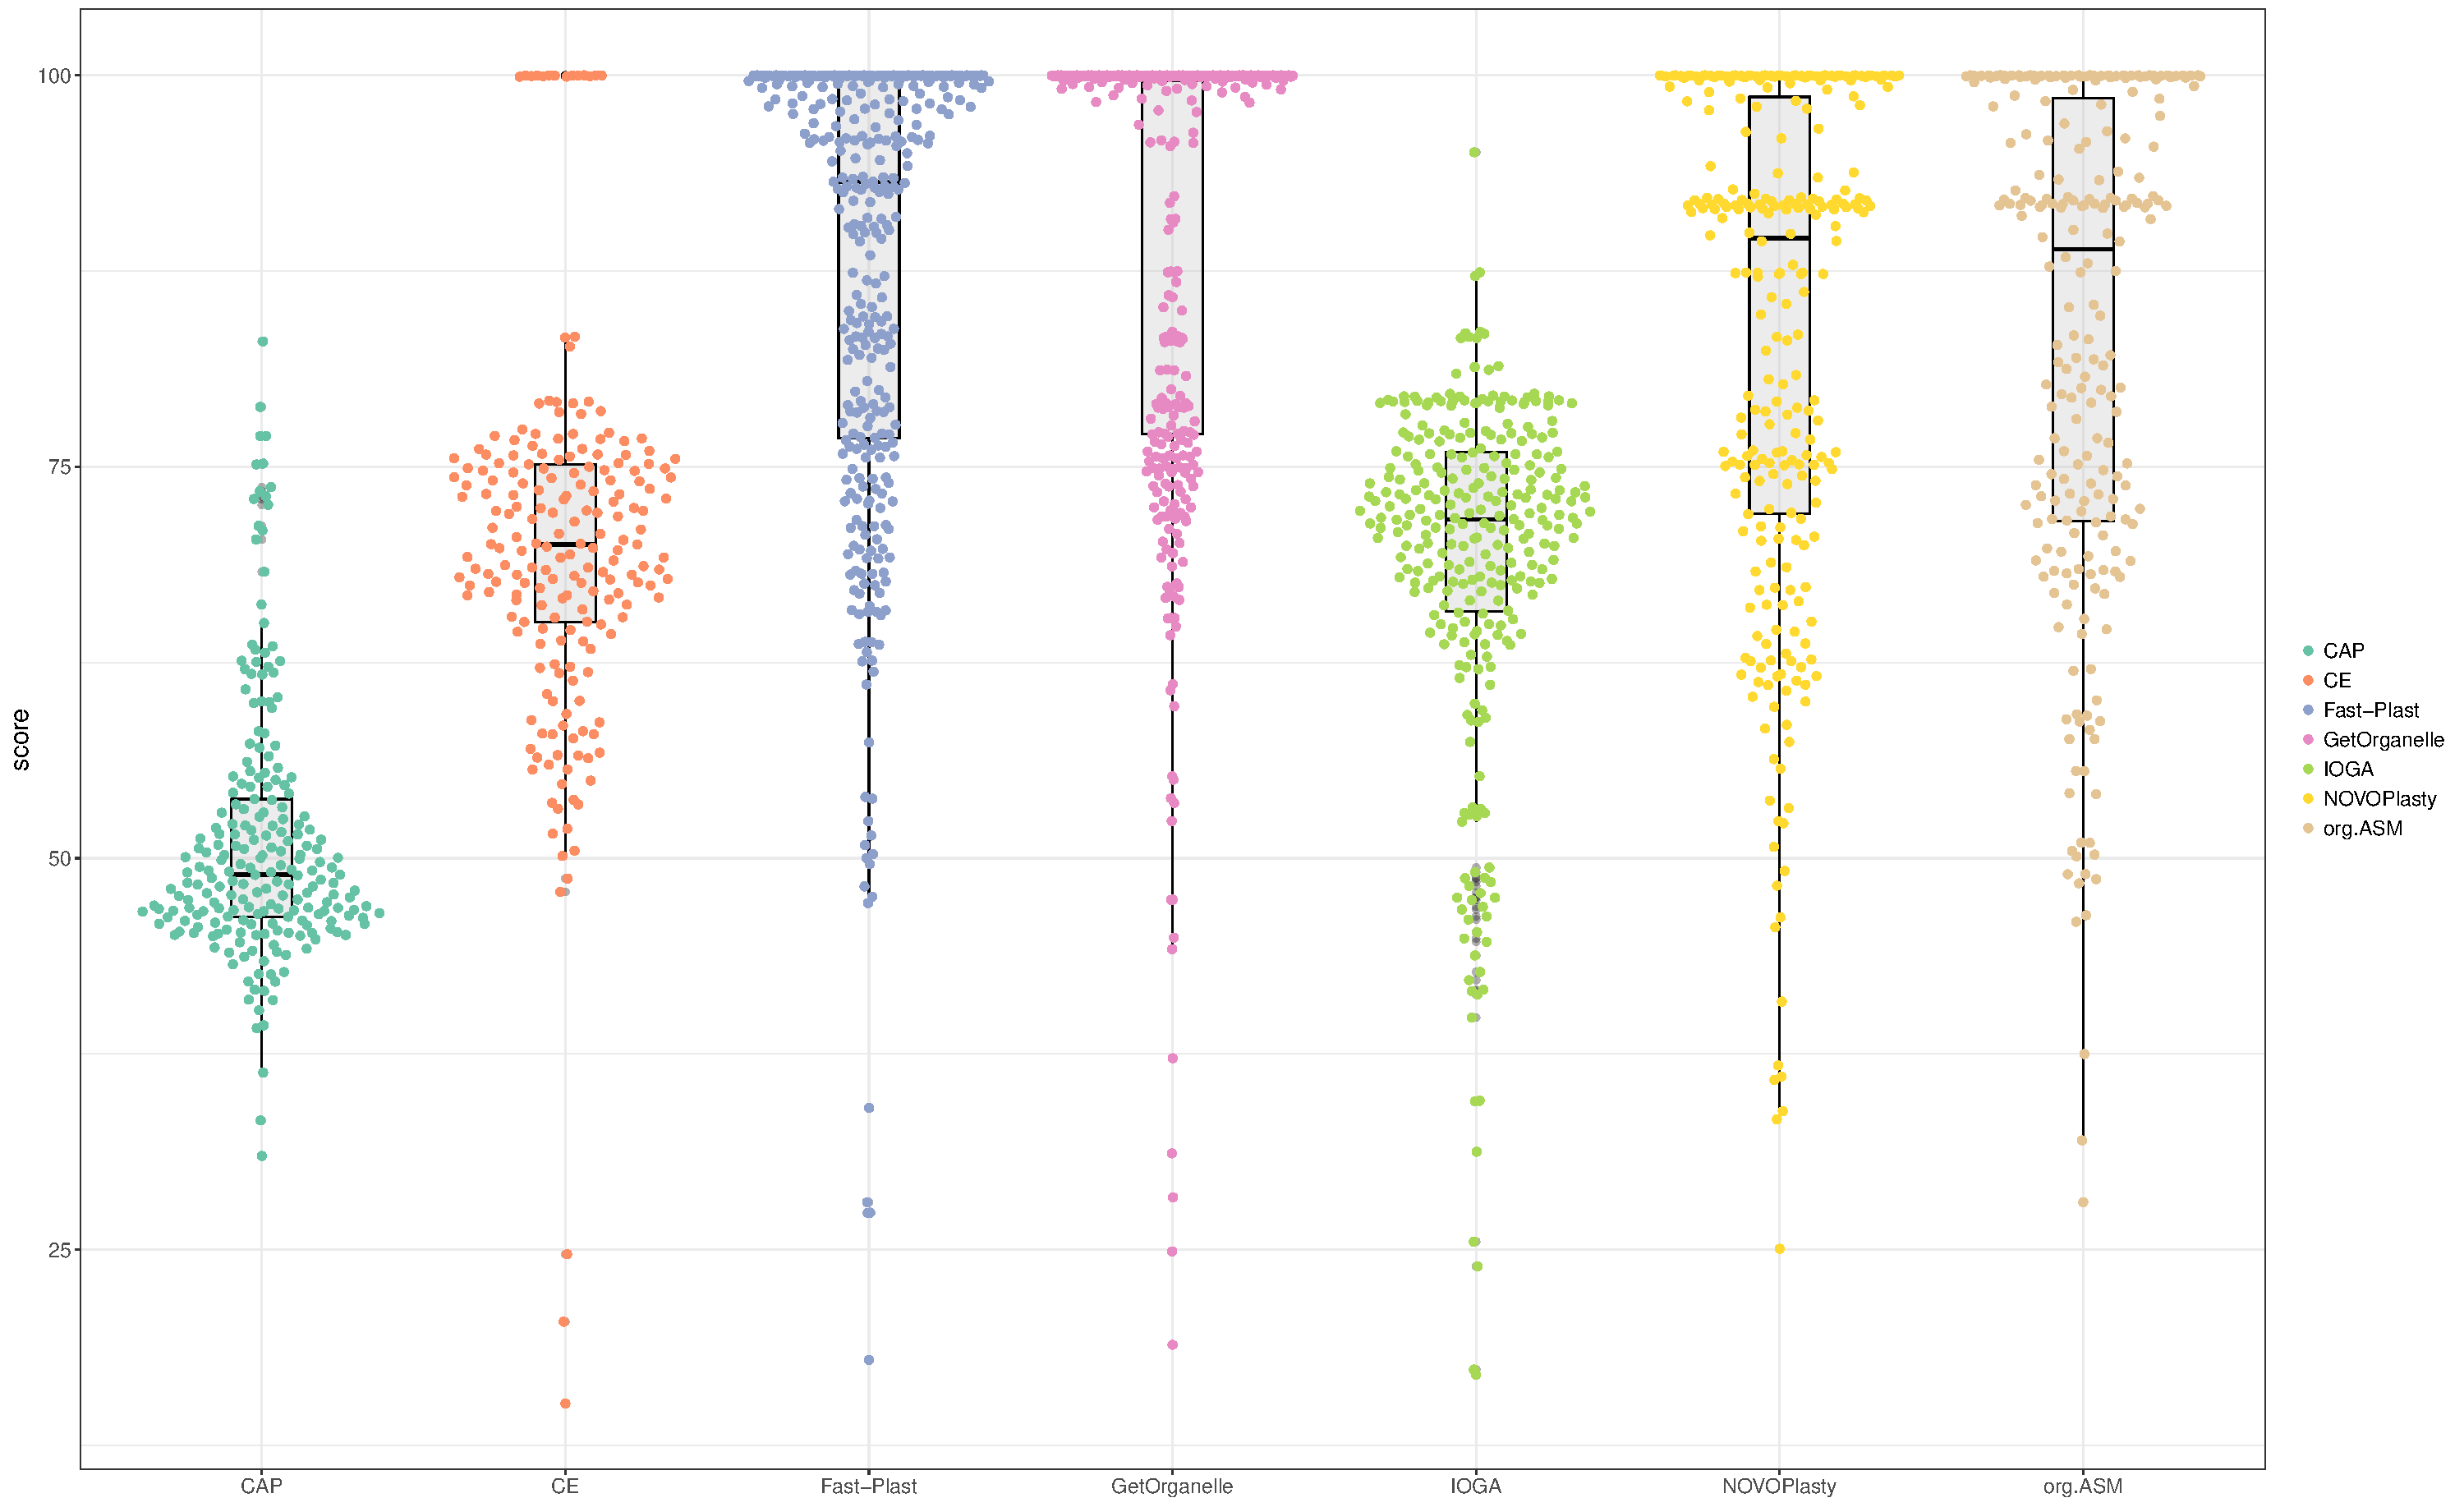
\includegraphics[width=\textwidth]{plots/swarm.pdf}
  \caption{\csentence{Sample figure title.}
      A short description of the figure content
      should go here.}
      \label{fig:swarmplot}
      \end{figure}

\begin{figure}[h!]
  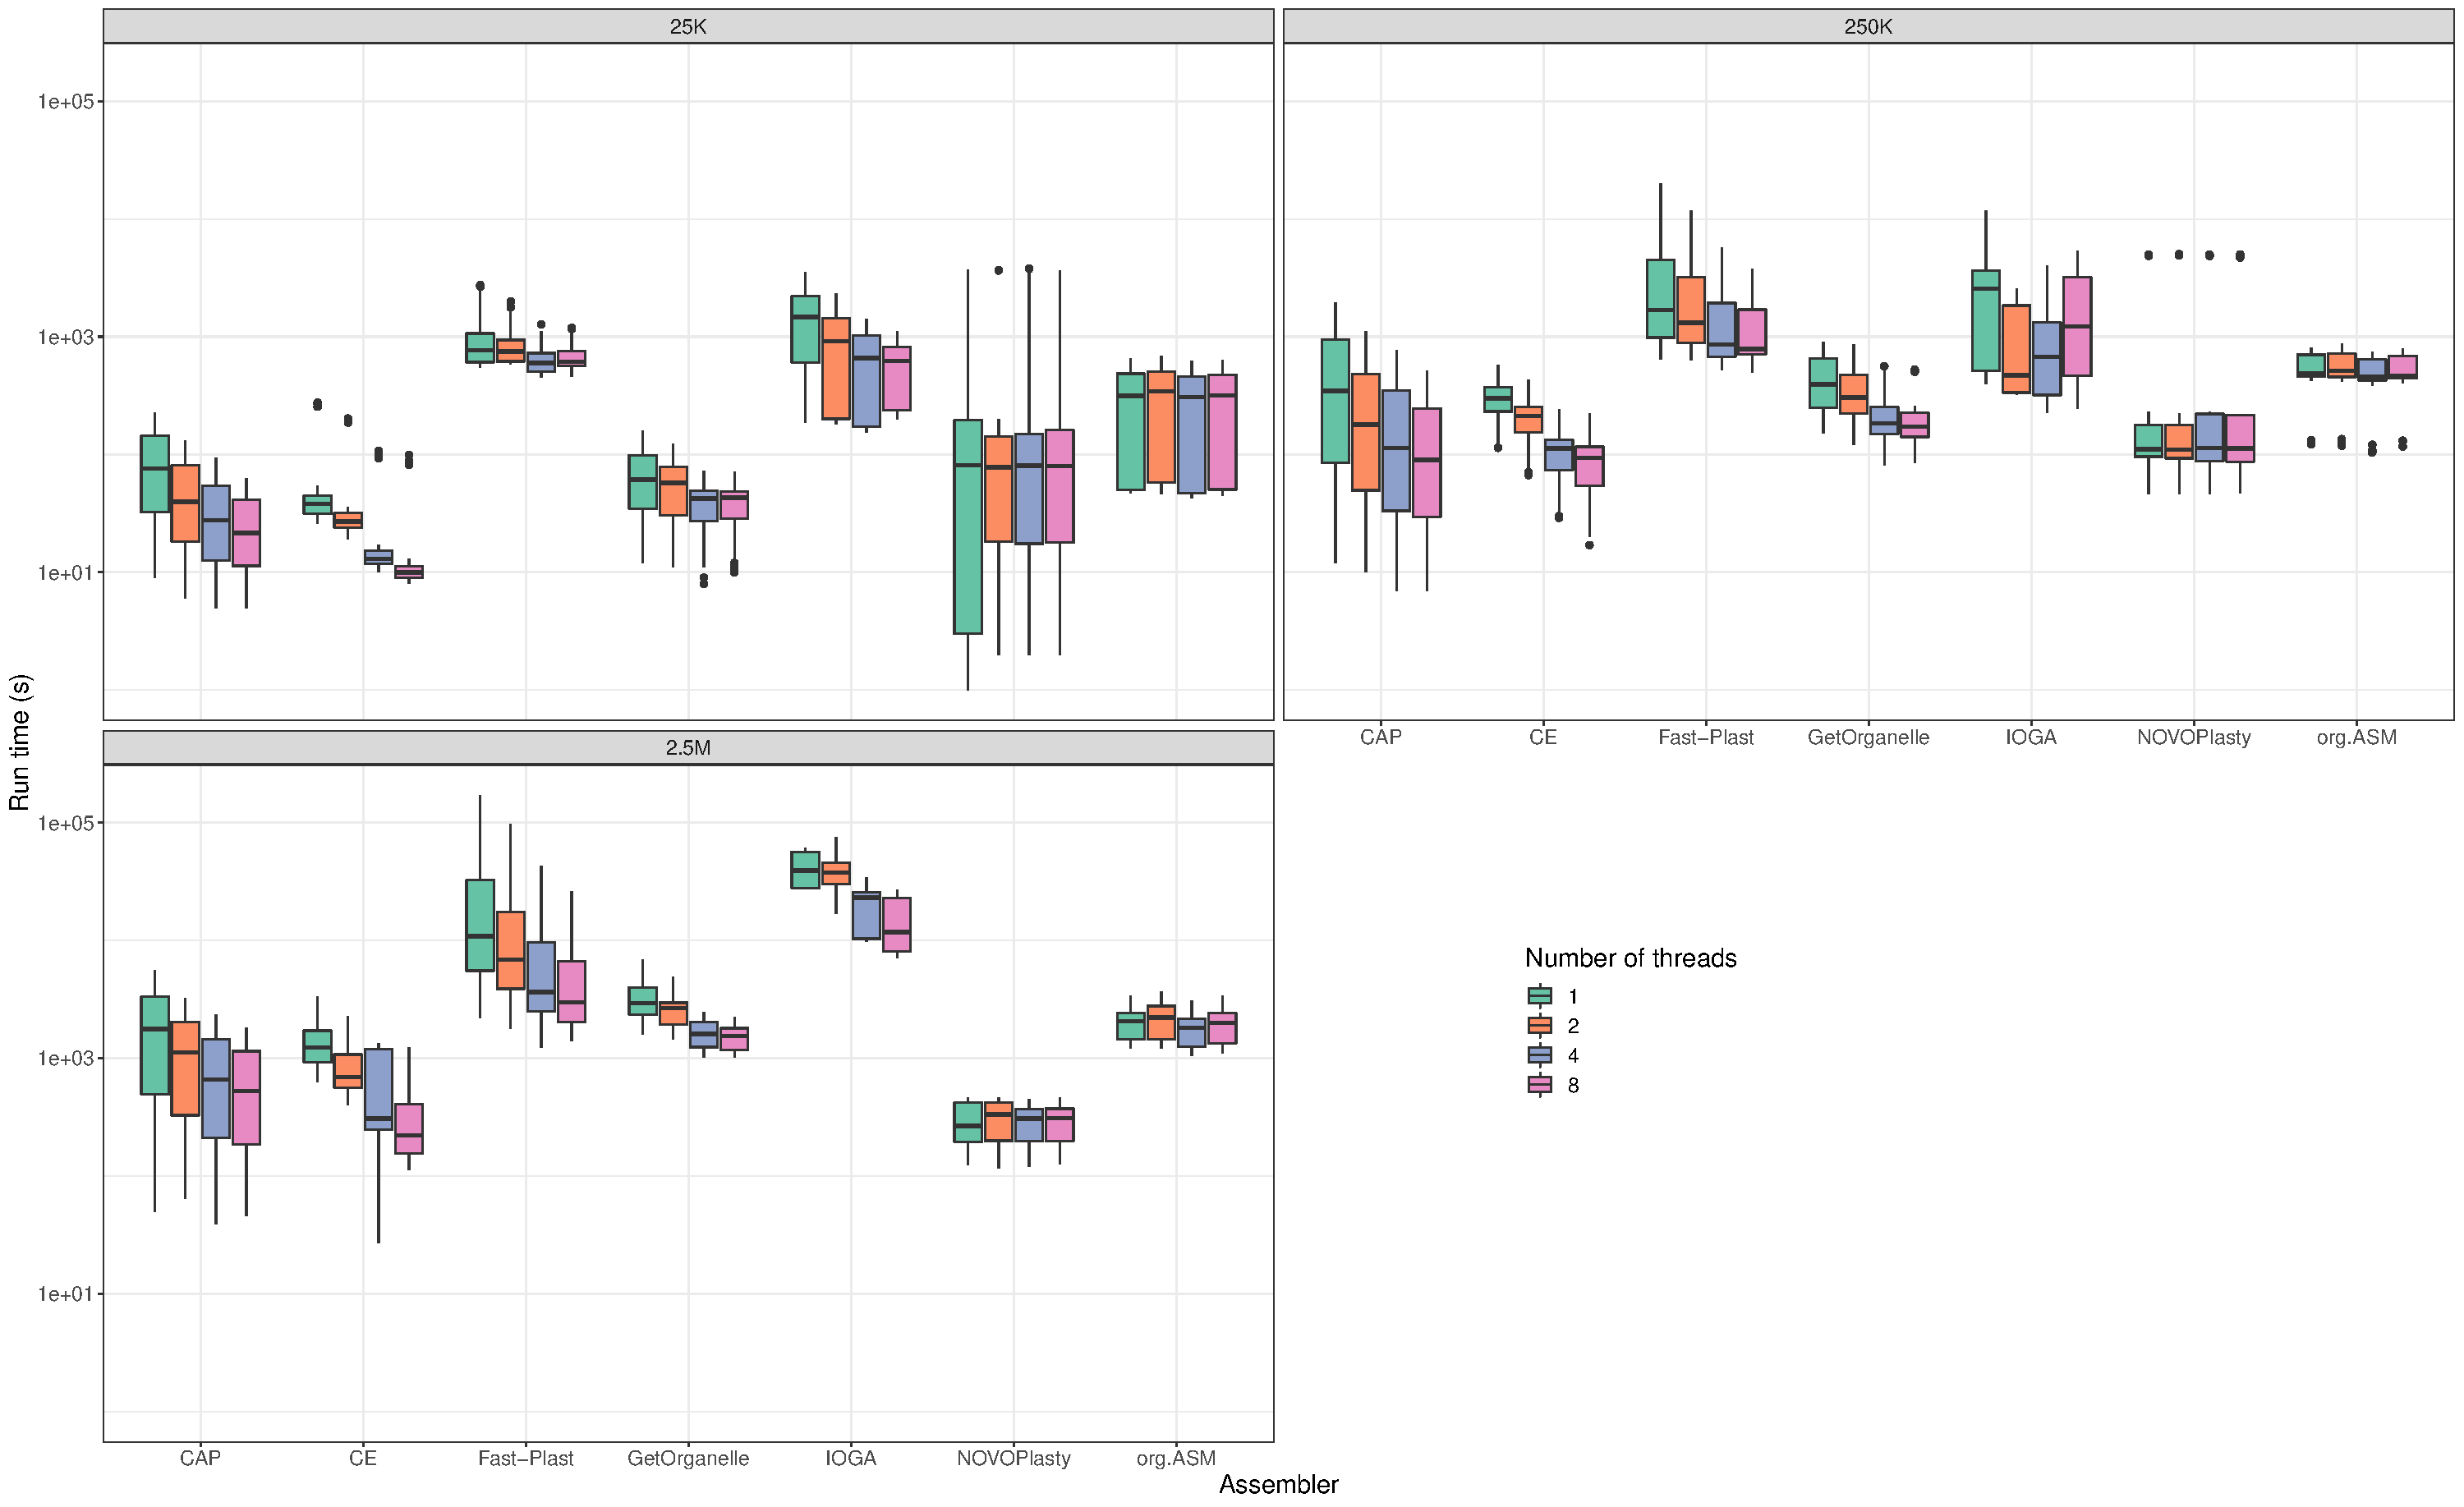
\includegraphics[width=\textwidth]{plots/comp_time_log.pdf}
  \caption{\csentence{Computation time depending on number of threads and size of input data}
  }
        \label{fig:performance_runtime}
      \end{figure}

\begin{figure}[h!]
  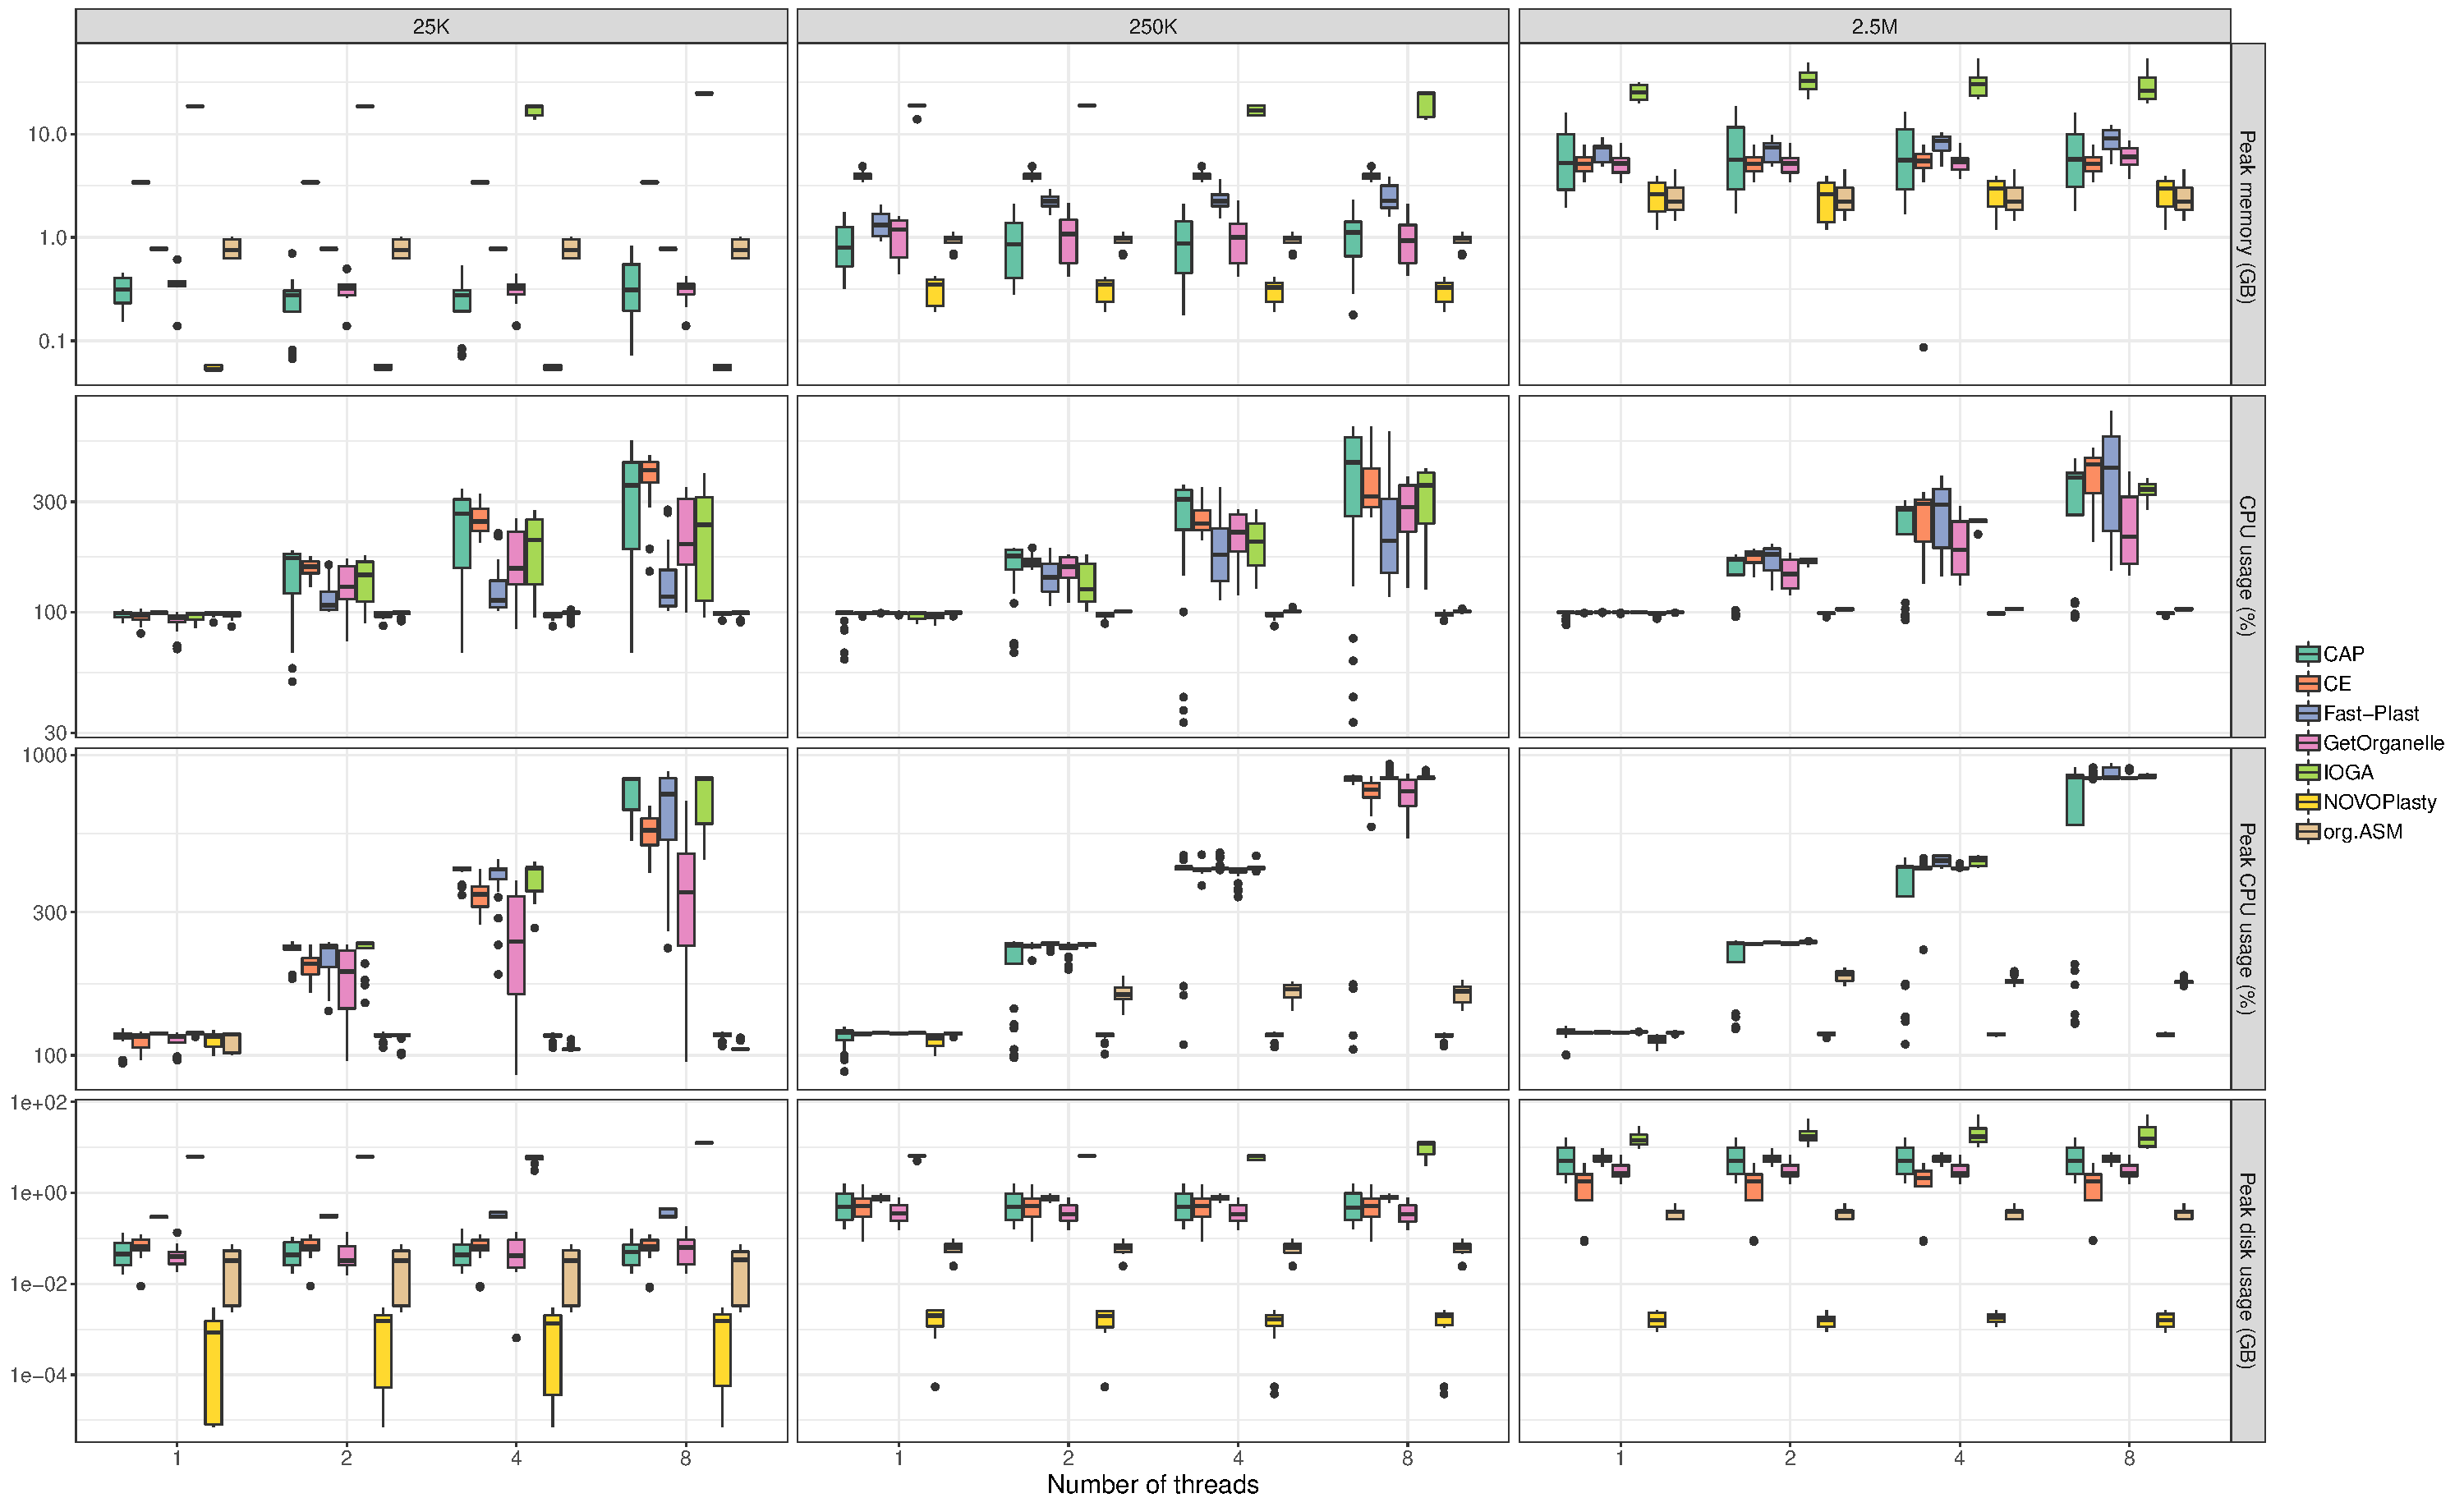
\includegraphics[width=\textwidth]{plots/usage_amount_threads.pdf}
  \caption{\csentence{Performance metrics}
      Boxplots depictiing the demand of CPU and RAM and disk space needed depending on the assembler, input data size and number of threads}
      \label{fig:performance_memory_cpu}
      \end{figure}

\begin{figure}[h!]
  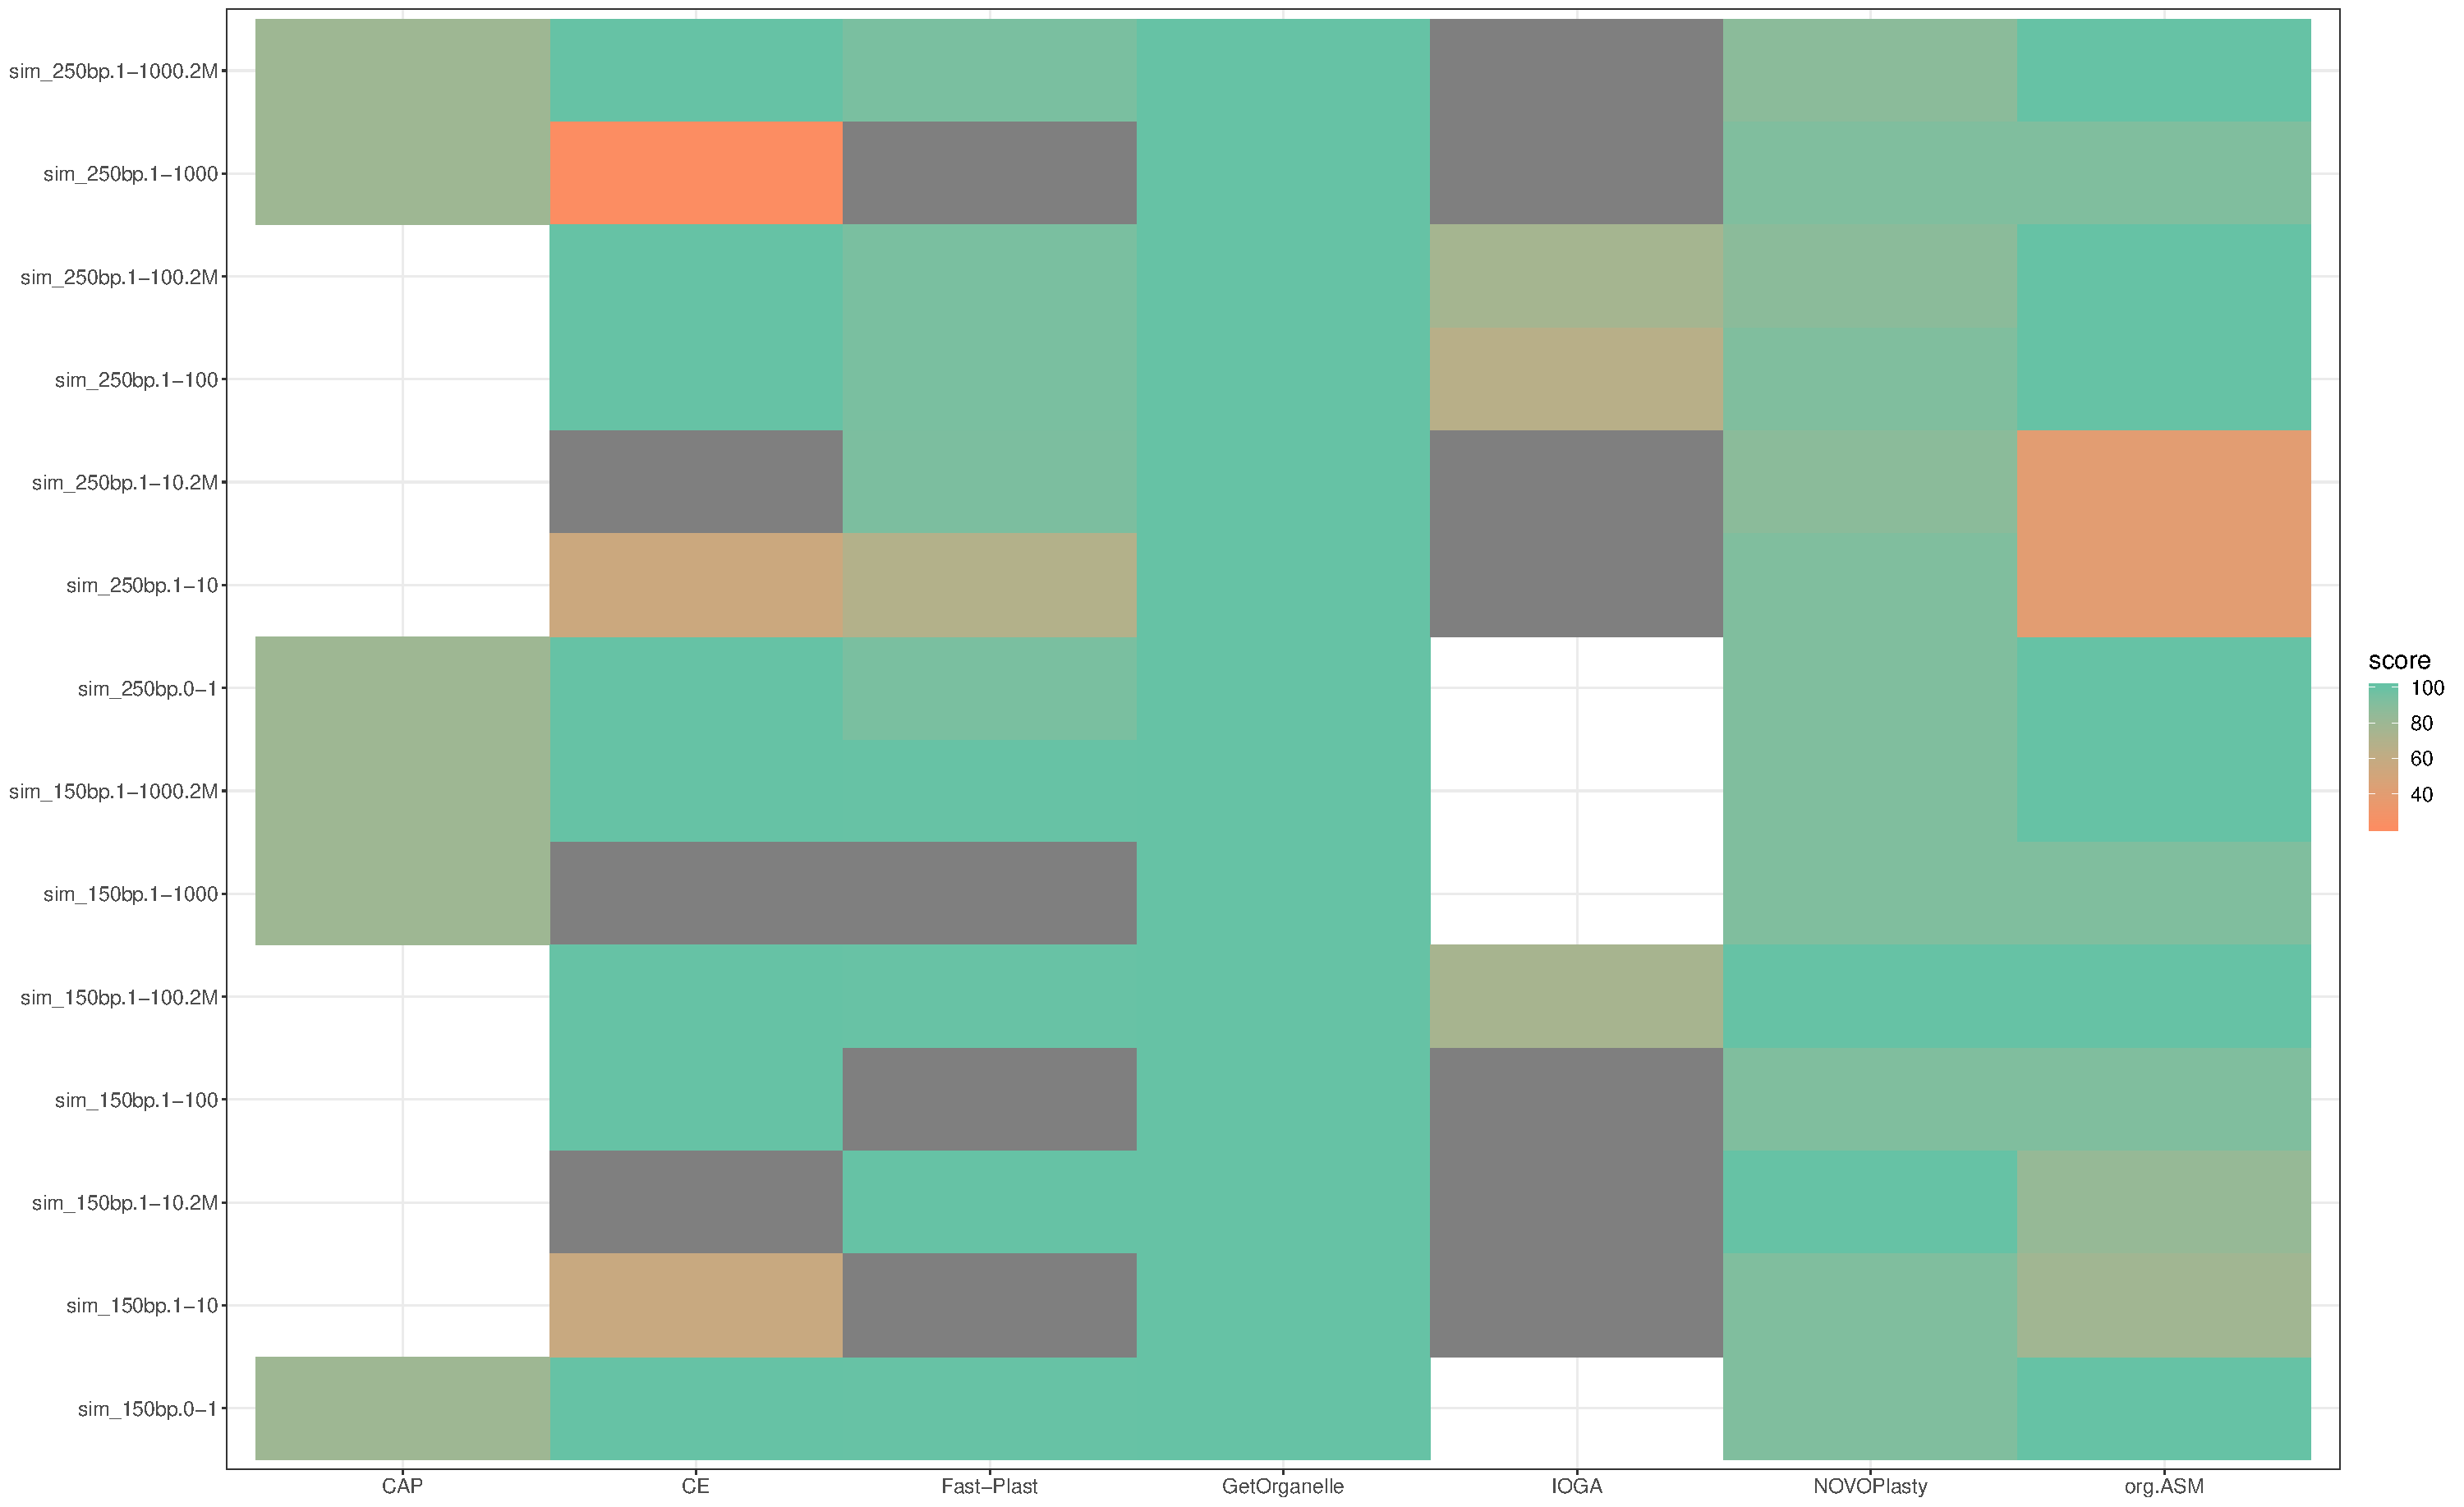
\includegraphics[width=\textwidth]{plots/sim_tiles.pdf}
  \caption{\csentence{Score of assemblies on simulated data}
      Figure legend text.}
      \label{fig:simulated}
      \end{figure}

\begin{figure}[h!]
  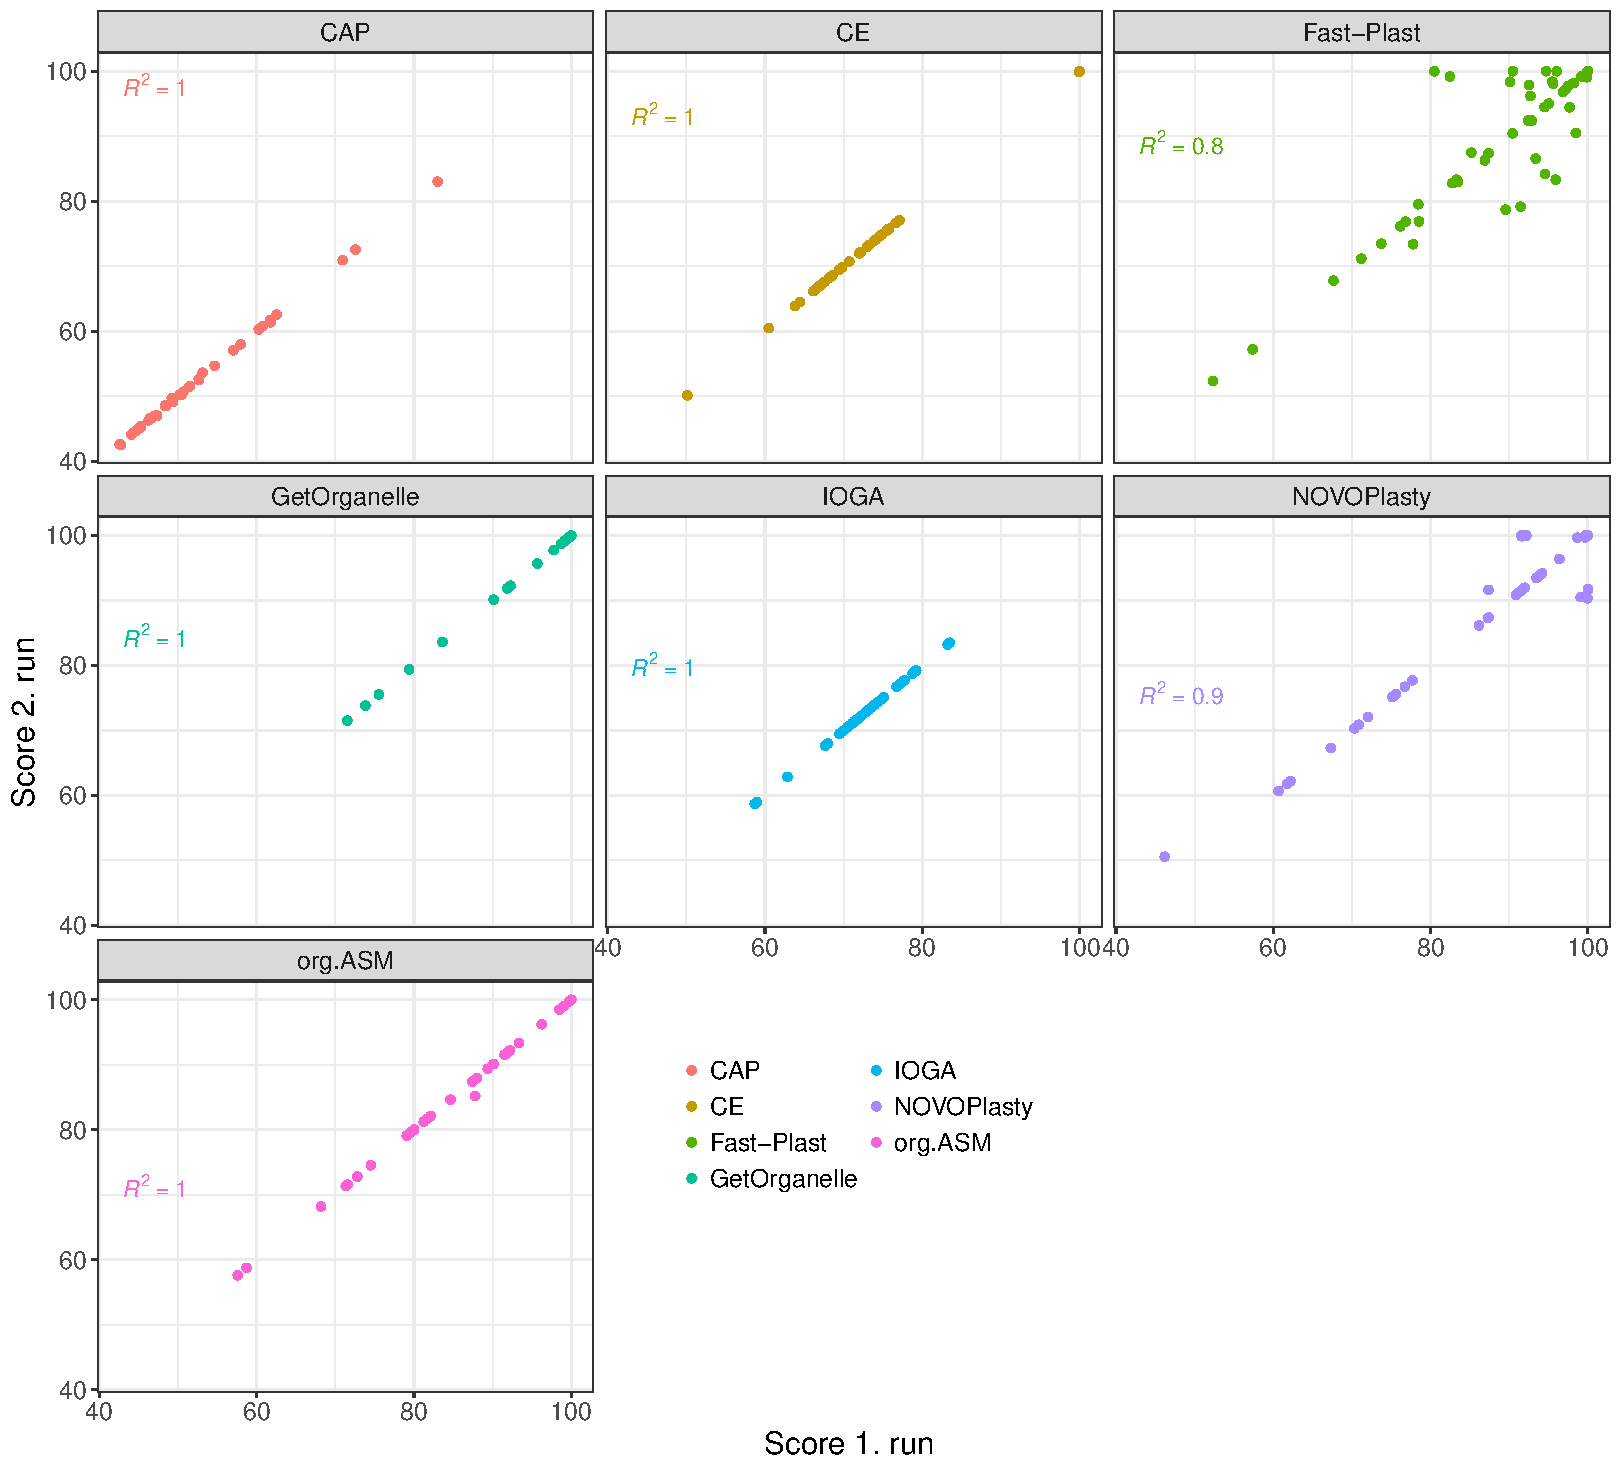
\includegraphics[width=\textwidth]{plots/repro.pdf}
  \caption{\csentence{Scores between two independent runs for reproducibility testing}
      }
      \label{fig:reproducibility}
      \end{figure}

\begin{figure}[h!]
  
\includegraphics[width=\textwidth,page=2]{plots/upset.pdf}
  \caption{\csentence{Upset plot \cite{lex2014upset} comparing success of assemblers on the real data sets}
      The plot shows the intersection of success ($score > 99$) between assemblers. For \num{69} datasets only \go{} was able to obtain a complete chloroplast. \num{43} were successful with both \go{} and \fp{} and so on}
            \label{fig:upset}
      \end{figure}

\begin{figure}[h!]
  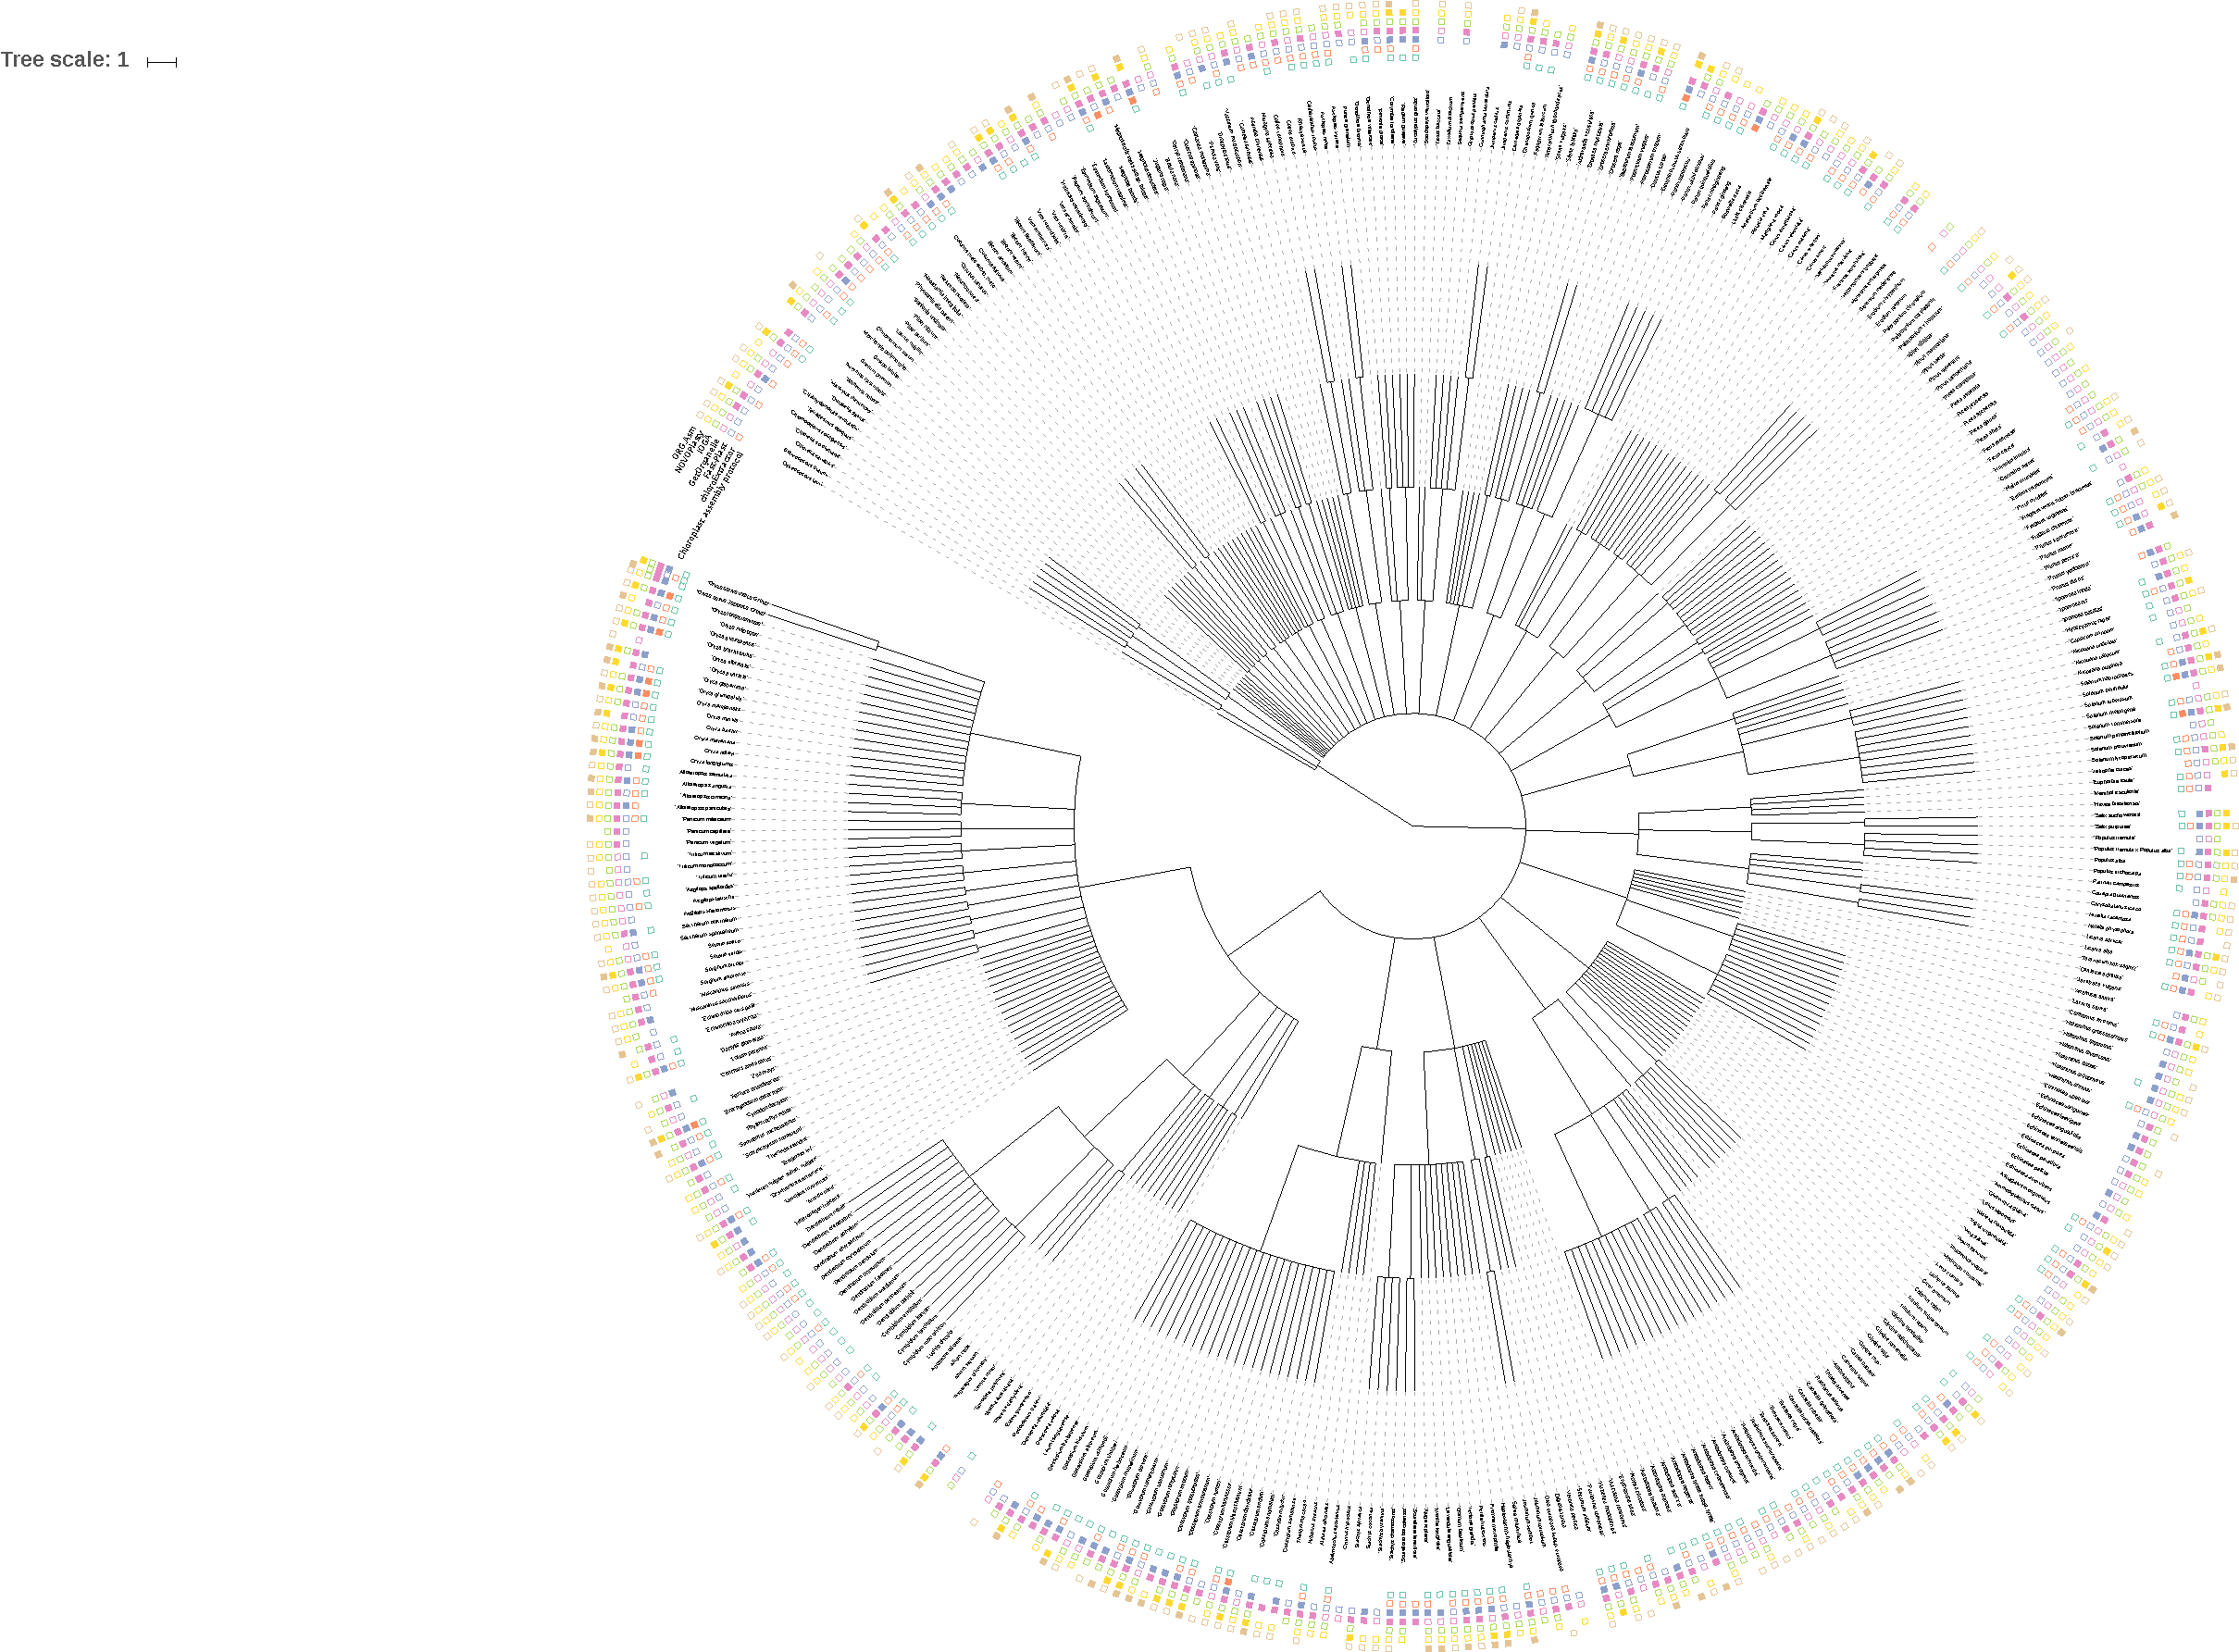
\includegraphics[width=\textwidth]{plots/real_datasets_tree.pdf}
  \caption{\csentence{Sucess of assemblers on real data sets on tree derived from ncbi taxonomy \cite{ncbi2011}}
      Figure legend text.}
      \label{fig:tree}
      \end{figure}

%%%%%%%%%%%%%%%%%%%%%%%%%%%%%%%%%%%
%%                               %%
%% Tables                        %%
%%                               %%
%%%%%%%%%%%%%%%%%%%%%%%%%%%%%%%%%%%

%% Use of \listoftables is discouraged.
%%
\section*{Tables}
\begin{table}[]
    \centering
    \caption{Overview of the results of the qualitative usability evaluation. Each tool 
    could score \good{}, \ok{} or \bad{} in each of the categories.}
    \label{tab:resultsQual}
\begin{tabular}{p{3cm}cccccc}   
Tool & Installation & Test/Tutorial & Documentation & Maintenance & FLOSS\\                           \hline \ce{}     &  \good{}  &  \good{}  &  \good{}  &  \good{}  &  \good{} \\
\cassp{}  &  \ok{}    &  \good{}  &  \ok{}    &  \good{}  &  \good{} \\
\fp{}     &  \bad{}   &  \ok{}    &  \good{}  &  \good{}  &  \good{} \\
\go{}     &  \ok{}    &  \ok{}    &  \good{}  &  \good{}  &  \good{} \\
\ioga{}   &  \bad{}   &  \bad{}   &  \ok{}    &  \ok{}    &  \bad{}  \\
\np{}     &  \good{}  &  \good{}  &  \good{}  &  \good{}  &  \ok{}   \\
\oa{}     &  \bad{}   &  \bad{}   &  \ok{}    &  \good{}  &  \good{} \\ \hline
\end{tabular}      
\end{table}

\begin{table}[h!]
\caption{Docker images used in our benchmark setup.}
\label{tab:dockerimages}
\centering
      \resizebox{\textwidth}{!}{\begin{tabular}{ccc}
        \hline
          Tool & Image name and tag & SHA256 Checksum   \\ \hline
          \ce & \dockerce & \dockercesha \\
          \cassp & \dockercassp & \dockercasspsha \\
          \fp & \dockerfp & \dockerfpsha \\
          \go & \dockergo & \dockergosha \\
          \ioga & \dockerioga & \dockeriogasha \\
          \np & \dockernp & \dockernpsha \\
          \oa & \dockeroa & \dockeroasha \\ \hline
      \end{tabular}}
\end{table}


\begin{table}[ht]
\caption{Mean scores of chloroplast genome assemblers}
\label{tab:scores}
\centering
\begin{tabular}{rlrrrr}
  \hline
 & assembler & Mean & SD & N\_perfect & N\_tot \\ 
  \hline
  1 & CAP & 51.26 & 8.42 &   0 & 221 \\ 
  2 & CE & 69.99 & 12.33 &  14 & 205 \\ 
  3 & Fast-Plast & 86.96 & 15.33 & 114 & 352 \\ 
  4 & GetOrganelle & 89.13 & 15.30 & 199 & 356 \\ 
  5 & IOGA & 68.74 & 11.69 &   0 & 296 \\ 
  6 & NOVOPlasty & 82.78 & 16.55 &  66 & 270 \\ 
  7 & org.ASM & 82.77 & 16.38 &  55 & 228 \\ 
   \hline
\end{tabular}
\end{table}


\begin{table}[ht]
\caption{Performance metrics input size 25K}
\label{tab:perform25K}
\centering
\begin{tabular}{rlrrrr}
  \hline
 & program & threads & Peak CPU usage & Peak memeory & Peak disk usage (GB) \\ 
  \hline
1 & CAP &   1 & 113.32 & 0.31 & 0.06 \\ 
  2 & CAP &   2 & 166.60 & 0.26 & 0.05 \\ 
  3 & CAP &   4 & 305.99 & 0.26 & 0.05 \\ 
  4 & CAP &   8 & 569.12 & 0.37 & 0.06 \\ 
  5 & CE &   1 & 111.49 & 3.41 & 0.07 \\ 
  6 & CE &   2 & 199.12 & 3.41 & 0.07 \\ 
  7 & CE &   4 & 343.22 & 3.41 & 0.07 \\ 
  8 & CE &   8 & 509.51 & 3.41 & 0.07 \\ 
  9 & Fast-Plast &   1 & 118.31 & 0.77 & 0.30 \\ 
  10 & Fast-Plast &   2 & 213.57 & 0.77 & 0.31 \\ 
  11 & Fast-Plast &   4 & 379.27 & 0.77 & 0.32 \\ 
  12 & Fast-Plast &   8 & 657.20 & 0.77 & 0.35 \\ 
  13 & GetOrganelle &   1 & 111.39 & 0.38 & 0.05 \\ 
  14 & GetOrganelle &   2 & 170.30 & 0.32 & 0.05 \\ 
  15 & GetOrganelle &   4 & 242.27 & 0.31 & 0.06 \\ 
  16 & GetOrganelle &   8 & 346.98 & 0.31 & 0.07 \\ 
  17 & IOGA &   1 & 118.12 & 18.61 & 6.25 \\ 
  18 & IOGA &   2 & 224.74 & 17.88 & 6.26 \\ 
  19 & IOGA &   4 & 394.98 & 16.62 & 5.60 \\ 
  20 & IOGA &   8 & 733.11 & 21.76 & 11.13 \\ 
  21 & NOVOPlasty &   1 & 78.38 & 0.04 & 0.00 \\ 
  22 & NOVOPlasty &   2 & 86.64 & 0.04 & 0.00 \\ 
  23 & NOVOPlasty &   4 & 86.50 & 0.04 & 0.00 \\ 
  24 & NOVOPlasty &   8 & 87.32 & 0.04 & 0.00 \\ 
  25 & org.ASM &   1 & 112.08 & 0.79 & 0.03 \\ 
  26 & org.ASM &   2 & 115.44 & 0.79 & 0.03 \\ 
  27 & org.ASM &   4 & 105.09 & 0.79 & 0.03 \\ 
  28 & org.ASM &   8 & 105.78 & 0.79 & 0.03 \\ 
   \hline
\end{tabular}
\end{table}

\begin{table}[ht]
\caption{Performance metrics input size 250K}
\label{tab:perform250K}
\centering
\begin{tabular}{rlrrrr}
  \hline
 & program & threads & Peak CPU usage & Peak memeory & Peak disk usage (GB) \\ 
  \hline
1 & CAP &   1 & 114.38 & 0.90 & 0.65 \\ 
  2 & CAP &   2 & 204.39 & 0.93 & 0.65 \\ 
  3 & CAP &   4 & 337.09 & 0.97 & 0.65 \\ 
  4 & CAP &   8 & 652.75 & 1.08 & 0.65 \\ 
  5 & CE &   1 & 117.57 & 3.96 & 0.63 \\ 
  6 & CE &   2 & 230.35 & 3.96 & 0.63 \\ 
  7 & CE &   4 & 414.25 & 3.96 & 0.63 \\ 
  8 & CE &   8 & 755.76 & 3.97 & 0.63 \\ 
  9 & Fast-Plast &   1 & 118.81 & 1.40 & 0.78 \\ 
  10 & Fast-Plast &   2 & 234.12 & 2.25 & 0.78 \\ 
  11 & Fast-Plast &   4 & 425.89 & 2.32 & 0.79 \\ 
  12 & Fast-Plast &   8 & 845.94 & 2.52 & 0.79 \\ 
  13 & GetOrganelle &   1 & 117.94 & 1.07 & 0.40 \\ 
  14 & GetOrganelle &   2 & 227.05 & 1.13 & 0.40 \\ 
  15 & GetOrganelle &   4 & 403.35 & 1.08 & 0.40 \\ 
  16 & GetOrganelle &   8 & 747.20 & 1.03 & 0.39 \\ 
  17 & IOGA &   1 & 118.62 & 12.03 & 4.01 \\ 
  18 & IOGA &   2 & 234.09 & 9.71 & 4.01 \\ 
  19 & IOGA &   4 & 420.77 & 10.09 & 3.48 \\ 
  20 & IOGA &   8 & 842.57 & 19.21 & 9.45 \\ 
  21 & NOVOPlasty &   1 & 111.97 & 0.32 & 0.00 \\ 
  22 & NOVOPlasty &   2 & 115.07 & 0.32 & 0.00 \\ 
  23 & NOVOPlasty &   4 & 116.42 & 0.31 & 0.00 \\ 
  24 & NOVOPlasty &   8 & 115.86 & 0.31 & 0.00 \\ 
  25 & org.ASM &   1 & 118.10 & 0.93 & 0.06 \\ 
  26 & org.ASM &   2 & 161.76 & 0.93 & 0.06 \\ 
  27 & org.ASM &   4 & 163.01 & 0.93 & 0.06 \\ 
  28 & org.ASM &   8 & 160.74 & 0.93 & 0.06 \\ 
   \hline
\end{tabular}
\end{table}

\begin{table}[ht]
\caption{Performance metrics input size 2.5M}
\label{tab:perform2.5M  }
\centering
\begin{tabular}{rlrrrr}
  \hline
 & program & threads & Peak CPU usage & Peak memeory & Peak disk usage (GB) \\ 
 \hline
1 & CAP &   1 & 118.80 & 6.83 & 6.59 \\ 
  2 & CAP &   2 & 209.22 & 7.58 & 6.59 \\ 
  3 & CAP &   4 & 357.36 & 7.25 & 6.59 \\ 
  4 & CAP &   8 & 683.71 & 6.99 & 6.59 \\ 
  5 & CE &   1 & 118.78 & 5.34 & 2.01 \\ 
  6 & CE &   2 & 234.82 & 5.34 & 2.01 \\ 
  7 & CE &   4 & 415.74 & 5.28 & 2.09 \\ 
  8 & CE &   8 & 844.95 & 5.34 & 2.01 \\ 
  9 & Fast-Plast &   1 & 119.24 & 6.80 & 5.80 \\ 
  10 & Fast-Plast &   2 & 237.34 & 6.98 & 5.82 \\ 
  11 & Fast-Plast &   4 & 443.27 & 8.02 & 5.69 \\ 
  12 & Fast-Plast &   8 & 872.07 & 8.87 & 5.69 \\ 
  13 & GetOrganelle &   1 & 118.91 & 5.25 & 3.31 \\ 
  14 & GetOrganelle &   2 & 235.18 & 5.26 & 3.31 \\ 
  15 & GetOrganelle &   4 & 420.10 & 5.44 & 3.31 \\ 
  16 & GetOrganelle &   8 & 845.13 & 6.07 & 3.31 \\ 
  17 & IOGA &   1 & 119.46 & 18.64 & 8.83 \\ 
  18 & IOGA &   2 & 237.22 & 21.24 & 10.19 \\ 
  19 & IOGA &   4 & 425.50 & 18.71 & 10.56 \\ 
  20 & IOGA &   8 & 857.29 & 25.23 & 16.51 \\ 
  21 & NOVOPlasty &   1 & 112.67 & 2.69 & 0.00 \\ 
  22 & NOVOPlasty &   2 & 117.77 & 2.58 & 0.00 \\ 
  23 & NOVOPlasty &   4 & 117.40 & 2.74 & 0.00 \\ 
  24 & NOVOPlasty &   8 & 117.28 & 2.74 & 0.00 \\ 
  25 & org.ASM &   1 & 118.73 & 2.63 & 0.37 \\ 
  26 & org.ASM &   2 & 184.53 & 2.63 & 0.37 \\ 
  27 & org.ASM &   4 & 177.03 & 2.63 & 0.37 \\ 
  28 & org.ASM &   8 & 176.25 & 2.63 & 0.37 \\ 
   \hline
\end{tabular}
\end{table}


% \begin{table}[h!]
% \caption{Sample table title. This is where the description of the table should go.}
%       \begin{tabular}{cccc}
%         \hline
%           & B1  &B2   & B3\\ \hline
%         A1 & 0.1 & 0.2 & 0.3\\
%         A2 & ... & ..  & .\\
%         A3 & ..  & .   & .\\ \hline
%       \end{tabular}
% \end{table}

%%%%%%%%%%%%%%%%%%%%%%%%%%%%%%%%%%%
%%                               %%
%% Additional Files              %%
%%                               %%
%%%%%%%%%%%%%%%%%%%%%%%%%%%%%%%%%%%

\section*{Additional Files}
  \subsection*{Additional file 1 --- Sample additional file title}
    Additional file descriptions text (including details of how to
    view the file, if it is in a non-standard format or the file extension).  This might
    refer to a multi-page table or a figure.

  \subsection*{Additional file 2 --- Sample additional file title}
    Additional file descriptions text.


\end{backmatter}
\end{document}
